% Pacotes e configurações padrão do estilo "article"\
% -------------------------------------
\documentclass[a4paper,11pt,twocolumns]{article}
% Layout
% --------------------------------------------------------------------------------
\usepackage{pdfpages} % Pacote para inserir um PDF dentro do LaTeX
\usepackage{minted}
%     Gráficos e layout ----------------------------------------------------------------------

\ifx\pdfmatch\undefined
\else
    \usepackage[T1]{fontenc}
    \usepackage[utf8]{inputenc}
\fi
% xetex:
\ifx\XeTeXinterchartoks\undefined
\else
    \usepackage{fontspec}
    \defaultfontfeatures{Ligatures=TeX}
\fi
% luatex:
\ifx\directlua\undefined
\else
    \usepackage{fontspec}
    \DeclareTextCommand{\nobreakspace}{T1}{\leavevmode\nobreak\ } % Fix Problems with caption
    \usepackage{luacode} % Permite usar o ambiente luacode
\fi
% End engine-specific settings

%      Fonte --------------------------------------------------------------------------------
%\usepackage{lmodern}
\usepackage{times}
%     Pacotes adicionados -------------------------------------------------------------------
\usepackage{ae}
%     Língua e hifenização ------------------------------------------------------------------
\usepackage[portuguese]{babel}
\usepackage{hyphenat}
%      Outros --------------------------------------------------------------------------------
\usepackage{fancyhdr}
\usepackage{sectsty}
\usepackage{float}
%\usepackage{graphicx}
%\usepackage[pdftex]{color,graphicx}
\usepackage{hyperref}
\usepackage{enumerate} % Permite alterar Layout do enumerate
\usepackage{pdflscape} % Permite alterar a orientação da pagina usando o ambiente landscape
%\usepackage{ifthen} % Permite usar condicionais ifelse
%\usepackage[table]{xcolor} % Permite alterar as cores das celulas de uma tabela
\usepackage{amsmath,amssymb} % Ambiente para uso de elementos matemáticos
\usepackage{caption}
\usepackage{subcaption} % permite o uso de multiplas figuras com legenda
\usepackage{minted} % FOrmatador para códigos de programas
\usepackage{natbib} % Para referencia bibliográfica
\usepackage{url} % pacote url
% Layout do documento ------------------------------------------------------------------------
%     Bordas e tamanho da página ------------------------------------------------------------
\usepackage{geometry} 
 \geometry{ % Padrõa ABNT para relatórios
 a4paper,
 left=30mm,
 right=20mm,
 top=30mm,
 bottom=20mm
 }
%     Cabeçalho e Rodapé ---------------------------------------------------------------
\pagestyle{fancy}
  \lhead{}
  \chead{}
  \rhead{}
  \lfoot{}
  \cfoot{}
  \rfoot{\thepage}
%     Númeração ------------------------------------------------------------------------
  \pagenumbering{arabic}
%     Retas do cabeçalho e rodapé ------------------------------------------------------
  \renewcommand{\headrulewidth}{0.5pt}
  \renewcommand{\footrulewidth}{0.5pt}
%     Tamanho da letra de seções e derivadas --------------------------------------------
  \sectionfont{\normalsize}
  \subsectionfont{\small}
%     Hiperlinks ------------------------------------------------------------------------
  \hypersetup{
                  colorlinks,
                  citecolor=black,
                  filecolor=black,
                  linkcolor=black,
                  urlcolor=black
                  }
%     Dados do título e autores --------------------------------------------------------------
%\title{\tituloRelatorio}
\author{Rafael Lima}
%     Definições do pdf ----------------------------------------------------------------------
\hypersetup{
    unicode=false,          % non-Latin characters in Acrobat’s bookmarks
    pdftoolbar=true,        % show Acrobat’s toolbar?
    pdfmenubar=true,        % show Acrobat’s menu?
    pdffitwindow=false,     % window fit to page when opened
    pdfstartview={FitH},    % fits the width of the page to the window    
    pdfauthor={Rafael Lima},     % author
    pdfnewwindow=true      % links in new window
}
%     Outros ----------------------------------------------------------------------------
      %\renewcommand{\thesection}{(\alph{section})} % muda o estilo de númeração das sections
      % alterando a formatação dos numeradores de lista de itens
      \renewcommand\theenumi{\arabic{enumi}}
      \renewcommand\labelenumi{(\textit{\theenumi})}
	  \renewcommand\theenumii{\arabic{enumii}}
	  \renewcommand\labelenumii{(\textit{\theenumi.\theenumii})}
      
% ---------------------------------------------------------------------------------------

\newcommand{\tituloRelatorio}{Prova 2}
\title{\tituloRelatorio}
\hypersetup{pdftitle={\tituloRelatorio}}% title
% Definições Auxiliares
% -----------------------------------------------------------------
%\input{relat_aux.tex}
% ----------------------------------~>ø<~---------------------------------------
\begin{document}
% Capa e Índice ---------------------------------------------------------------
%--------------------------------------------------- Capa --------------------------------------------
%\newpage
\begin{flushleft}
Universidade de Brasilia - UnB\\
Departamento de Ciências da Computação - CIC\\
Disciplina: Programação em Tempo Real\\
%Professor: 
\end{flushleft}

\vspace{0.3\textheight}
\begin{center}
    \Huge\textbf{\\\tituloRelatorio \\}
\end{center}

\vspace{0.3\textheight}
\begin{flushleft}
\textbf{Aluno:}\\
\vspace{2mm}
\begin{tabular}{ll}
    Rafael Lima & 10/0131093
\end{tabular}
%Professor: 
\end{flushleft}

%\thispagestyle{empty} % Retira o cabeçalho e o rodapé da página

% ------------------------------------------------- Índice -------------------------------------------
\newpage
\tableofcontents
\newpage
% ----------------------------------------------------------------------------------------------------



% Conteúdo -------------------------------------------------------------------
\section{Introdução}
No presente projeto, foi feito o estudo, modelagem e análise de um processo automatizado de manufatura descrito em um vídeo. O processo analisado foi o demonstração da FANUC de montagem rápida de chave de carro com sistema de alarme utilizando dois robôs Pick'n'Place. Disponível no link \url{https://www.youtube.com/watch?v=GqrSYDNVXw8&feature=youtu.be&list=PLECC02EA2EAE0E159}\ .

 Neste processo é necessário a sincronia de 5 sistemas de maneira concorrente para o perfeito funcionamento, representando os agentes dentro do processo. São estes a Esteira, o Robô 1 (encarregado de posicionar a bateria e tampa), o disco aonde são posicionadas as chaves, o robô 2 ( encarregado de parafusar a tampa) e a caixa de parafusos ( local aonde são fornecidos os parafusos para montagem ). Para tal foi utilizado a descrição do sistema em liguagem $CSP_m$. Permitindo assim a análise no computador do processo de maneira independente da forma de sua implementação.

\subsection{Disco}
O disco representa o elemento integrador de toda a linha de montagem, têm movimento contínuo e por ele a chave percorre ao longo de todo o processo. Inicialmente a chave chega desmontada e a partir de cada etapa são acrescentadas as demais peças pelos robôs situados a esquerda e a direita do vídeo. Similar a outros modelo comumente encontrado em linhas de montagem de produção baseados em esteiras.

\subsection{Esteira}
A esteira atua fornecendo uma bateria e uma tampa para o robô 1. Diferentemente do disco, sua movimentação é alternada entre momentos parada e momentos em movimento. Inicialmente a esteira move trazendo um par de peças para a posição aonde o robô 1 deve pegar e aguarda. Assim que o robô 1 pega a peça, uma câmera detecta o espaço vazio deixado após ambas peças serem removidas e torna a mover a esteira.

\subsection{Robô 1}
O robô 1 é responsável por posicionar a bateria e em seguida a tampa da chave. Para tal, ele atua em sincronismo com a esteira pegando a bateria e em seguida pegando a tampa, de modo que a todo momento que retorna a posição inicial têm uma nova tampa e uma nova bateria disponível. As peças são colocadas na chave com o disco em movimento, sendo tal ponto destacado pelo fabricante como uma interpolação do movimento do robô em uma trajetória circular, feita em simetria com o movimento do disco. Desta forma, do ponto de vista da chave as peças são colocadas de cima para baixo enquanto esta se move pelo disco trazendo um ganho de tempo na montagem ao dispensar a parada para colocar cada peça.

\subsection{Robô 2}

O robô 2 é responsável por parafusar a tampa. Embora seja equipado com um atuador diferente, seu funcionamento é similar ao Robô 1. Ele busca um parafuso novo na Caixa de Parafuso e aciona o atuador com a parafusadeira enquanto o chave se move ao longo do disco, logo em seguida retorna a posição inicial para pegar um novo parafuso.

\subsection{Caixa Parafusos}
Para fornecer os parafusos ao Robô 2 existe uma caixa ao canto que fornecendo um parafuso por vez. A cada vez que um parafuso é retirado , outro é posicionado no mesmo lugar para o robô 2.

\section{Modelagem em CSP}
Para estudo do funcionamento do sistema foi modelado utilizando a sintaxe $CSP_m$, também chamado \textit{Machine Readable CSP}\cite{fdrManual} e avaliado dentro usando a ferramenta $FDR4$. Os arquivos completos com a implementação em CSP e acrescida do tempo encontram-se em anexo. Foram retirados trechos do código de cada arquivo e  cada parte do sistema, junto as suas próprias particularidades as quais foram descritas a seguir:

\subsection{Esteira}
Para modelar a esteira foi pensado o processo como duas esteiras em paralelo como movimento sincronizado. Desta forma a cada vez que a esteira movia desencadeava dois eventos representando a entrega da tampa e da bateria.

\begin{minted}[breaklines,frame=single]{lua}
-- Eventos
channel moveEsteira
channel bateriaDisponivel
channel bateriaLiberada
channel tampaDisponivel
channel tampaLiberada

-- Alfabeto de Eventos
aESTEIRA1 = {moveEsteira,bateriaDisponivel,bateriaLiberada}
aESTEIRA2 = {moveEsteira,tampaDisponivel,tampaLiberada}
aESTEIRA = {moveEsteira,bateriaDisponivel,bateriaLiberada,tampaDisponivel,tampaLiberada}

-- Processos
ESTEIRA1 = moveEsteira -> bateriaDisponivel -> bateriaLiberada -> ESTEIRA1
ESTEIRA2 = moveEsteira -> tampaDisponivel -> tampaLiberada -> ESTEIRA2
ESTEIRA = ESTEIRA1 [|{moveEsteira}|] ESTEIRA2
\end{minted}

\subsection{Robô 1}
O Robô 1 participa de duas etapas do processo de montagem: colocar a bateria e colocar a tampa da chave. Estas duas etapas são feitas com a chave em movimento sobre o disco. Para tal o robô têm que sincronizar sua movimentação com a trajetória da chave no disco ao mesmo tempo garantir a sincronia com a esteira na hora de pegar a bateria e a tampa. 

\begin{minted}[breaklines,frame=single]{lua}
-- eventos ROBO1
channel robo1Descanso,robo1PegaBateria,robo1ColocaBateria,robo1PegaTampa,robo1ColocaTampa

-- Alfabeto Robo 1
aROBO1 = {robo1Descanso,robo1PegaBateria,syncRobo1Bateria,robo1ColocaBateria,
          robo1PegaTampa,syncRobo1Tampa,robo1ColocaTampa}

-- Processo
ROBO1 = robo1Descanso -> bateriaDisponivel -> robo1PegaBateria -> bateriaLiberada 
       -> syncRobo1Bateria -> robo1ColocaBateria -> chaveComBateria
       -> tampaDisponivel -> robo1PegaTampa -> tampaLiberada
       -> syncRobo1Tampa -> robo1ColocaTampa -> chaveComTampa -> ROBO1
\end{minted}

\subsection{Disco}
O disco é o agente central do processo pelo qual a chave é deslocada ao longo de todas as etapas. Nele são dispostos várias chaves em estágios diferentes de montagem e sua movimentação é contínua. Para modelar no CSP foram identificado cada região do disco correspondente a cada estágio de montagem, desta forma os eventos são sempre vistos do ponto de vista de uma chave situada sobre o Disco. Para este trabalho a quantidade de chaves disponível é ignorada.

\begin{minted}[breaklines,frame=single]{lua}
-- Eventos relacionados ao objeto Chave
channel chaveVazia
channel chaveComBateria
channel chaveComTampa
channel chaveComParafuso
channel chavePronta

-- Evento Independente do disco
channel moveChaveComTampa

-- Eventos para Sincronismo com os Robos
channel syncRobo1Bateria
channel syncRobo1Tampa
channel syncRobo2Parafuso

-- Alfabeto do Disco
aDISCO = {chaveVazia, syncRobo1Bateria, chaveComBateria,
        chaveComTampa, moveChaveComTampa, syncRobo2Parafuso,
        chaveComParafuso, chavePronta}

-- Processo do Disco
DISCO = chaveVazia -> syncRobo1Bateria -> chaveComBateria -> syncRobo1Tampa
       -> chaveComTampa -> moveChaveComTampa -> syncRobo2Parafuso
       -> chaveComParafuso -> chavePronta -> DISCO
\end{minted}

\subsection{Robô 2}
O Robô 2 têm seu funcionamento similar o Robô 1. Sua função é pegar o parafuso disponível na Caixa de Parafuso e parafusar a tampa enquanto a chave mexe ao longo do disco. Desde modo, é necessário seu sincronismo com a Caixa de Parafusos, na espera da disponibilidade do parafuso, e com o Disco durante o processo de parafusamento do parafuso na tampa.

\begin{minted}[breaklines,frame=single]{lua}
-- Eventos relaciodos ao Robo 2
channel robo2Descanso, robo2PegaParafuso, apertaParafuso

-- Alfabeto do robô 2
aROBO2 = {robo2Descanso , parafusoDisponivel , robo2PegaParafuso,
         syncRobo2Parafuso , apertaParafuso ,chaveComParafuso}

-- Processo do Robô 2
ROBO2 = robo2Descanso -> moveChaveComTampa -> parafusoDisponivel -> robo2PegaParafuso -> parafusoLiberado
        -> syncRobo2Parafuso -> apertaParafuso -> chaveComParafuso
        -> ROBO2
\end{minted}

\subsection{Caixa Parafusos}
A Caixa de Parafusos foi modelada como um processo sequencial aonde a retirada de um parafuso desencadeia a chegada de um novo parafuso.

\begin{minted}[breaklines,frame=single]{lua}
-- Eventos da Caixa
channel caixaVazia, novoParafuso, parafusoDisponivel, parafusoLiberado

-- Alfabeto da Caixa
aCAIXA = {caixaVazia, novoParafuso, parafusoDisponivel,robo2PegaParafuso, parafusoLiberado}

-- Processo da Caixa
CAIXA = caixaVazia -> novoParafuso -> parafusoDisponivel
       -> parafusoLiberado -> CAIXA
\end{minted}


\subsection{Sincronizando os Processos}
Após modelar cada agente junto ao processo referente é necessário trabalhar o sincronismo entre as tarefas. A estratégia utilizada foi trabalhar o sincronismo 2 a 2 em 3 níveis. Primeiro foi sincronizado cada par de interação: o a esteira com o robõ 1, o robô 1 com o disco, o disco com o robô 2 e o robô 2 com a caixa de parafusos. Nesta etapa foram marcados os eventos comuns ao cada um dos agentes.

\begin{minted}[breaklines,frame=single]{lua}
SUBSISTEMA1 = ESTEIRA [|{bateriaDisponivel,bateriaLiberada,tampaDisponivel,tampaLiberada}|] ROBO1
SUBSISTEMA2 = ROBO1 [|{syncRobo1Bateria,syncRobo1Tampa,chaveComBateria,chaveComTampa}|] DISCO
SUBSISTEMA3 = DISCO [|{moveChaveComTampa,syncRobo2Parafuso,chaveComParafuso}|] ROBO2
SUBSISTEMA4 = ROBO2 [|{parafusoDisponivel,parafusoLiberado}|] CAIXA
\end{minted}

Deste modo os agentes acabam duplicados entre os sistemas. Para resolver isto, é feito uma nova sincronização entre dois subsistemas que compartilham o mesmo agente representando o sincronismo referente a ter a mesma entidade física realizando aquela sequência de eventos.

\begin{minted}[breaklines,frame=single]{lua}
SUBSISTEMA12 = SUBSISTEMA1 [|aROBO1|] SUBSISTEMA2
SUBSISTEMA23 = SUBSISTEMA2 [|aDISCO|] SUBSISTEMA3
SUBSISTEMA34 = SUBSISTEMA3 [|aROBO2|] SUBSISTEMA4
\end{minted}

Uma vez explicitado os pontos aonde são necessário o sincronismo. Basta colocar todos os processos em paralelo.

\begin{minted}[breaklines,frame=single]{lua}
SISTEMA = SUBSISTEMA12 [] SUBSISTEMA23 [] SUBSISTEMA34
\end{minted}

\subsection{Estudo Temporal}
O modelo original em CSP considera os eventos mas estes são assumidos de intervalos nulos entre si e de duração ignorada. Desta forma é permitido apenas sincronismo entre o início de dois eventos simultâneos ou ainda entre cadeias de eventos para que terminem e comecem ao mesmo tempo. No entanto, para algumas situações é necessário considerar o sincronismo, considerando um intervalo fixo de tempo antes, durante ou mesmo após a ocorrência do evento. Na abordagem tradicional este poderia ser modelado em uma aproximação como um evento intermediário de espera, tendo sua duração colocada apenas pela implementação real do sistema.

Uma outra abordagem, é entender o tempo decorrido em alguma transição pela quantidade de ciclos passados entre um instante considerado e outro. Neste entendimento, a percepção do tempo é dada por comparação entre um processo periódico com ciclos de duração constante e este é responsável pelo sincronismo de todo o sistema. Podemos entender este processo assim construído como nosso relógio. Como efeito, o relógio assim definido pode ser tão complexo como necessário, podendo representar unidades de tempo como um relógio de ponteiros com divisão de segundos, minutos e horas ou meramente uma transição entre dois estados como um conta gota.

\subsubsection{Modelagem do Relógio}
Para este trabalho, o relógio segue a ideia parecida com um conta gota. Temos um evento, denominado \textit{tock} dentro de um processo cíclico chamado relógio. A transição entre um \textit{tock} e outro representa a passagem de um ciclo do relógio. Esta abordagem é denominada \textit{tock-CSP}\cite{fdrManual}, logo, para o relógio temos:

\begin{minted}[breaklines,frame=single]{lua}
    CLOCK = tock -> CLOCK
\end{minted}

Com base nesta definição introduzida, um processo que começa sempre no contar do relógio poderia ser modelado como:
\begin{minted}[breaklines,frame=single]{lua}
    CONTAGEM = tock -> somaUm -> CONTAGEM [|tock|] CLOCK
\end{minted}

Por outro lado, para um processo que demora 4 ciclos do relógio, por exemplo, poderia ser modelado como:
\begin{minted}[breaklines,frame=single]{lua}
    PROCESSO_CURTO = eventoA -> eventoB -> PROCESSO_CURTO [] CLOCK_PROCESSO_CURTO
    CLOCK_PROCESSO_CURTO = tock->tock->tock->tock->CLOCK_PROCESSO_CURTO [|tock|] CLOCK
\end{minted}

A partir da implementação em FDR4, podemos ainda acrescentar a contagem de ciclos a partir de uma função recursiva, permitindo uma notação mais compacta:
\begin{minted}[breaklines,frame=single]{lua}
    delay(0,PROCESSO) = PROCESSO
    delay(1,PROCESSO) = tock -> PROCESSO
    delay(n,PROCESSO) = if n>0 then tock -> delay(n-1,PROCESSO) else error("Parâmetro Inválido")
\end{minted}

Deste modo, um relógio de ponteiro em um segundo demora exatamente um ciclo da contagem pode ser modelado na notação introduzida pela função recursiva como:
\begin{minted}[breaklines,frame=single]{lua}
    SEGUNDOS = tock -> SEGUNDOS [|tock|] CLOCK
    MINUTOS = delay(60,MINUTOS) [|tock|] CLOCK
    HORAS = delay(3600,HORAS) [|tock|] CLOCK
\end{minted}

Com base em tais conceitos apresentados, o modelo do sistema analisado foi acrescido do tempo a partir das mesmas abordagens introduzidas nos três exemplos anteriores em que tempos maiores de espera foram acrecidos uma quantidade de tock maior.

\section{Resultados}
\subsection{Esteira}
\begin{figure}[H]
    \centering
    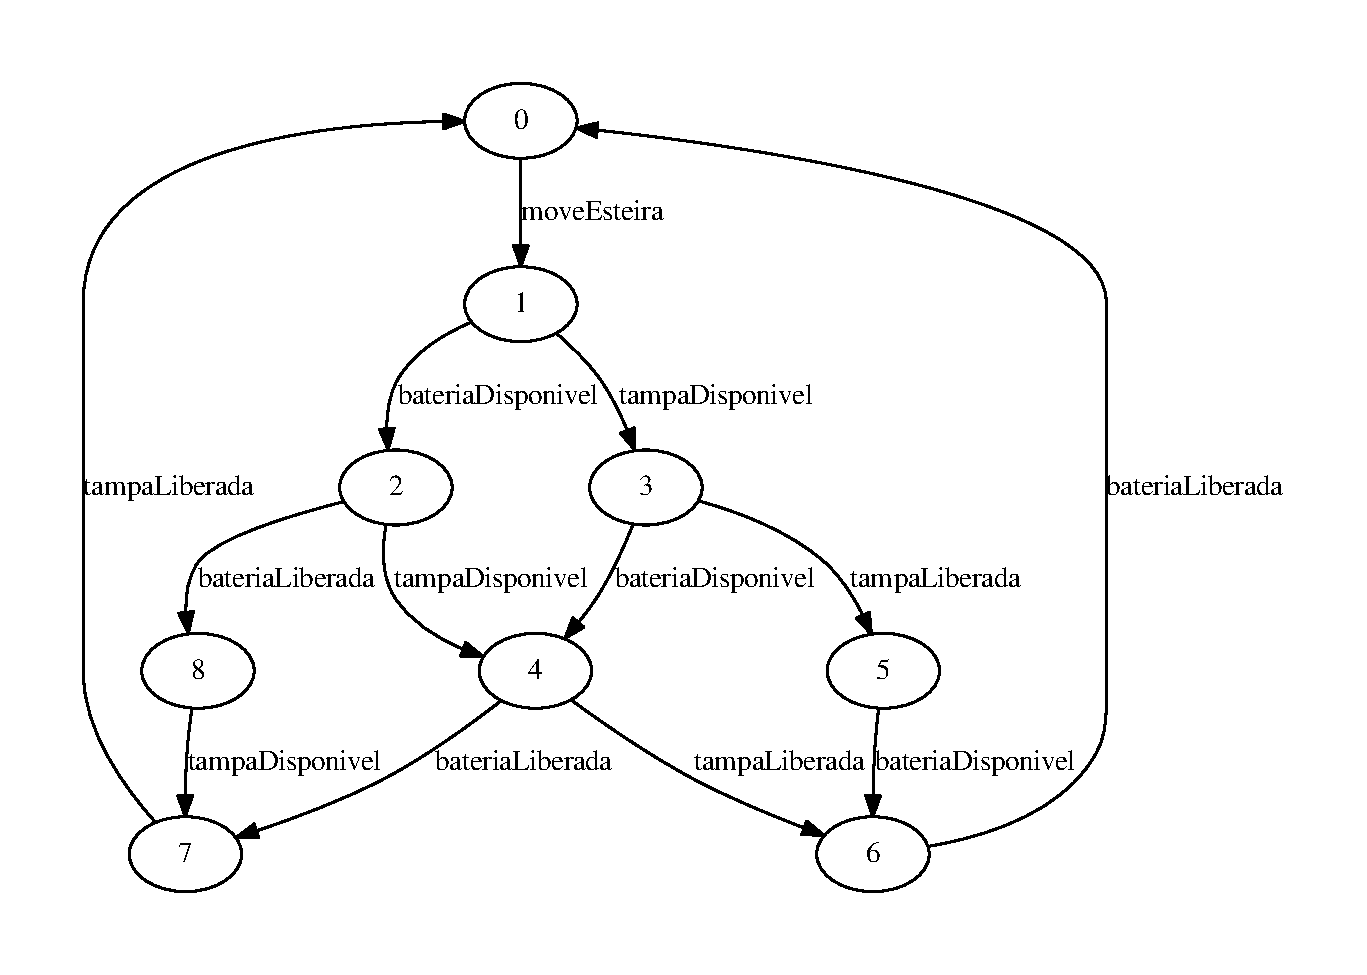
\includegraphics[width = 0.6\linewidth]{./img/g_esteira.pdf}
    \caption{Diagrama Esteira}
    \label{fig:g_esteira}
\end{figure}

\subsection{Caixa Parafusos}
\begin{figure}[H]
    \centering
    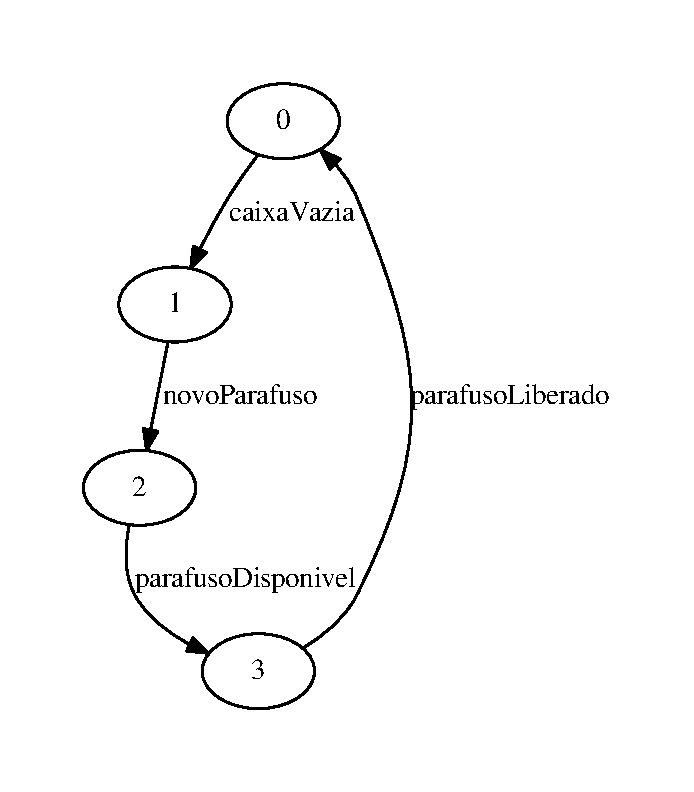
\includegraphics[width = 0.6\linewidth]{./img/g_caixa.pdf}
    \caption{Diagrama Caixa de Parafusos}
    \label{fig:g_caixa}
\end{figure}

\subsection{Disco}
\begin{figure}[H]
    \centering
    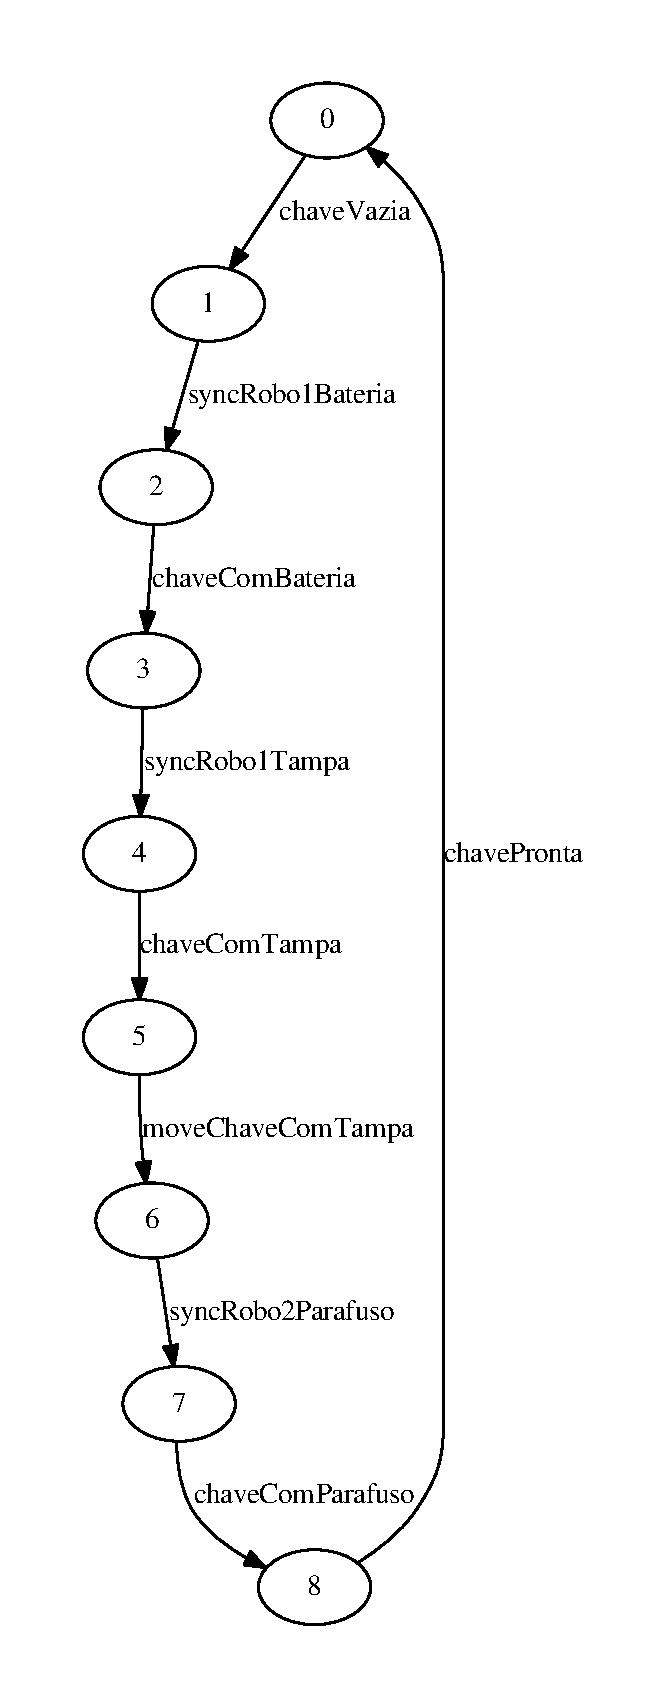
\includegraphics[height = 0.90\textheight]{./img/g_disco.pdf}
    \caption{Diagrama Disco}
    \label{fig:g_disco}
\end{figure}

\subsection{Robô 1}

\begin{figure}[H]
    \centering
    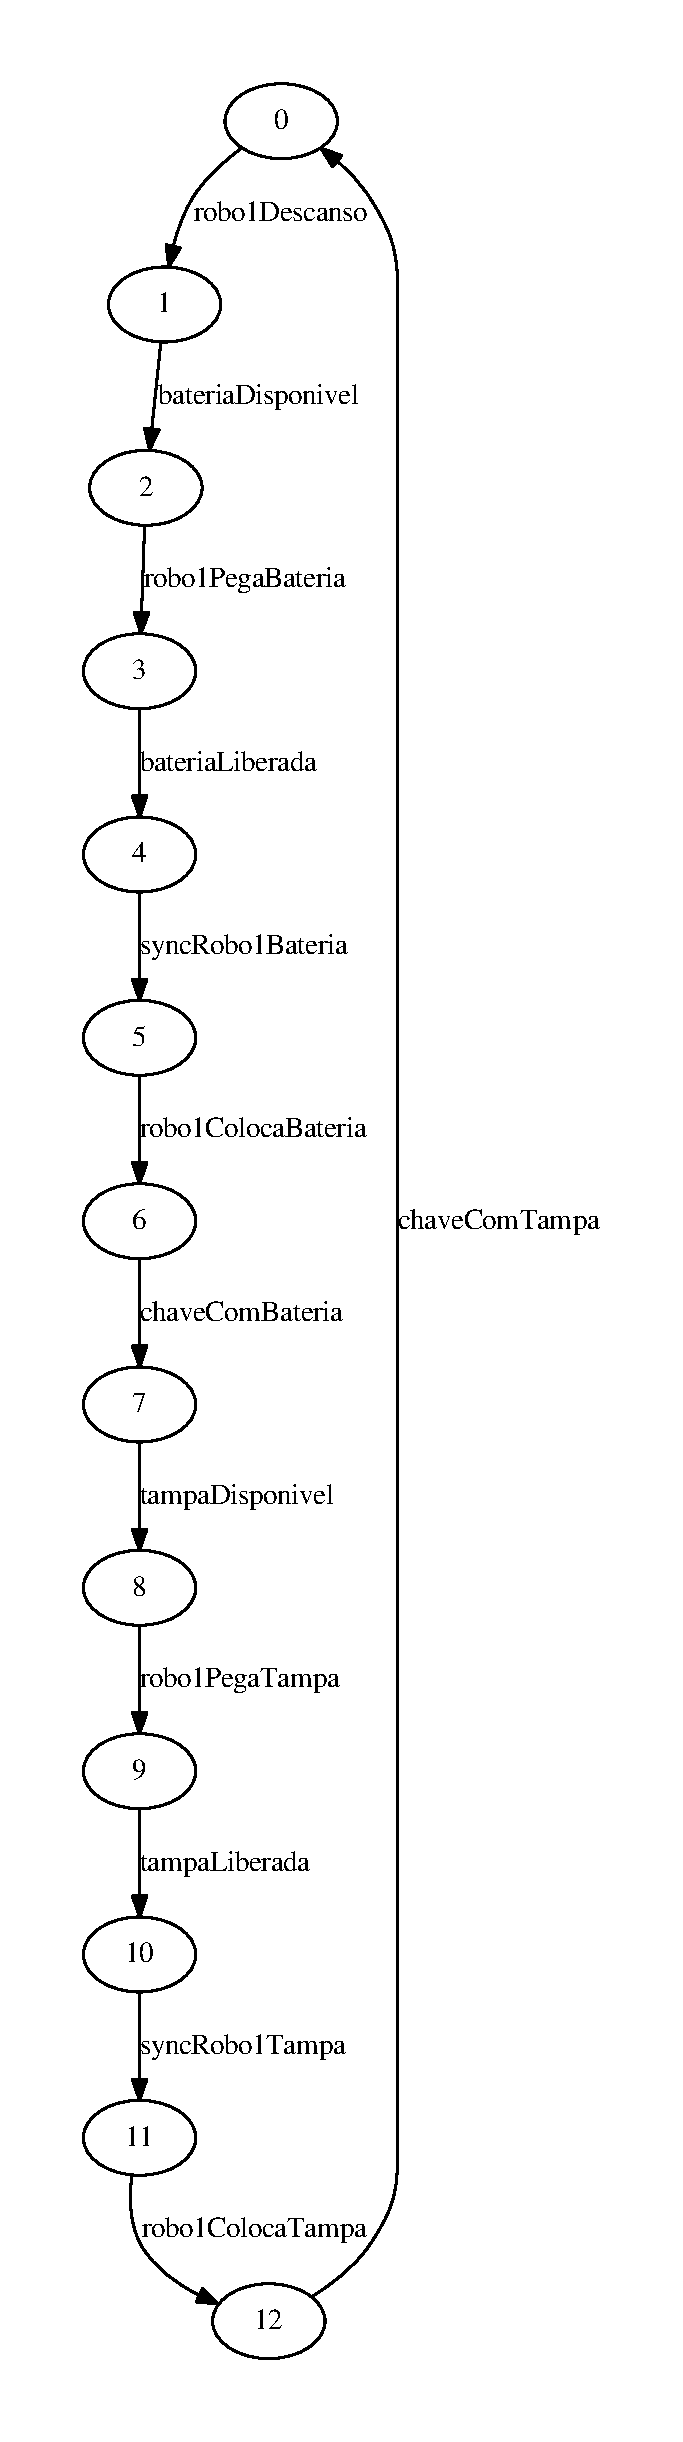
\includegraphics[height = 0.9\textheight]{./img/g_robo1.pdf}
    \caption{Diagrama Robô 1}
    \label{fig:g_robo1}
\end{figure}

\subsection{Robô 2}
\begin{figure}[H]
    \centering
    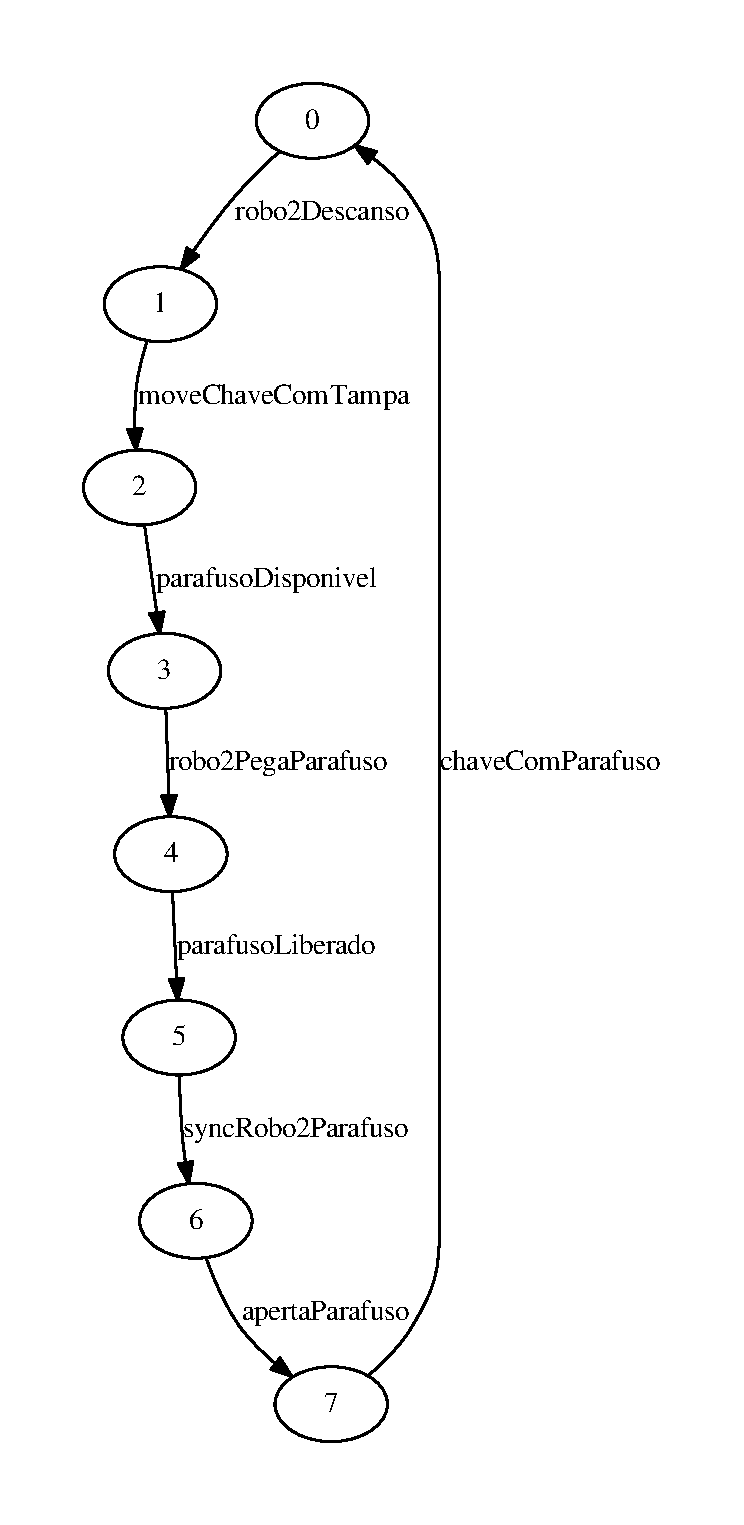
\includegraphics[height = 0.9\textheight]{./img/g_robo2.pdf}
    \caption{Diagrama Robô 2}
    \label{fig:g_robo2}
\end{figure}

\subsection{Subsistemas}
\begin{figure}[H]
    \centering
    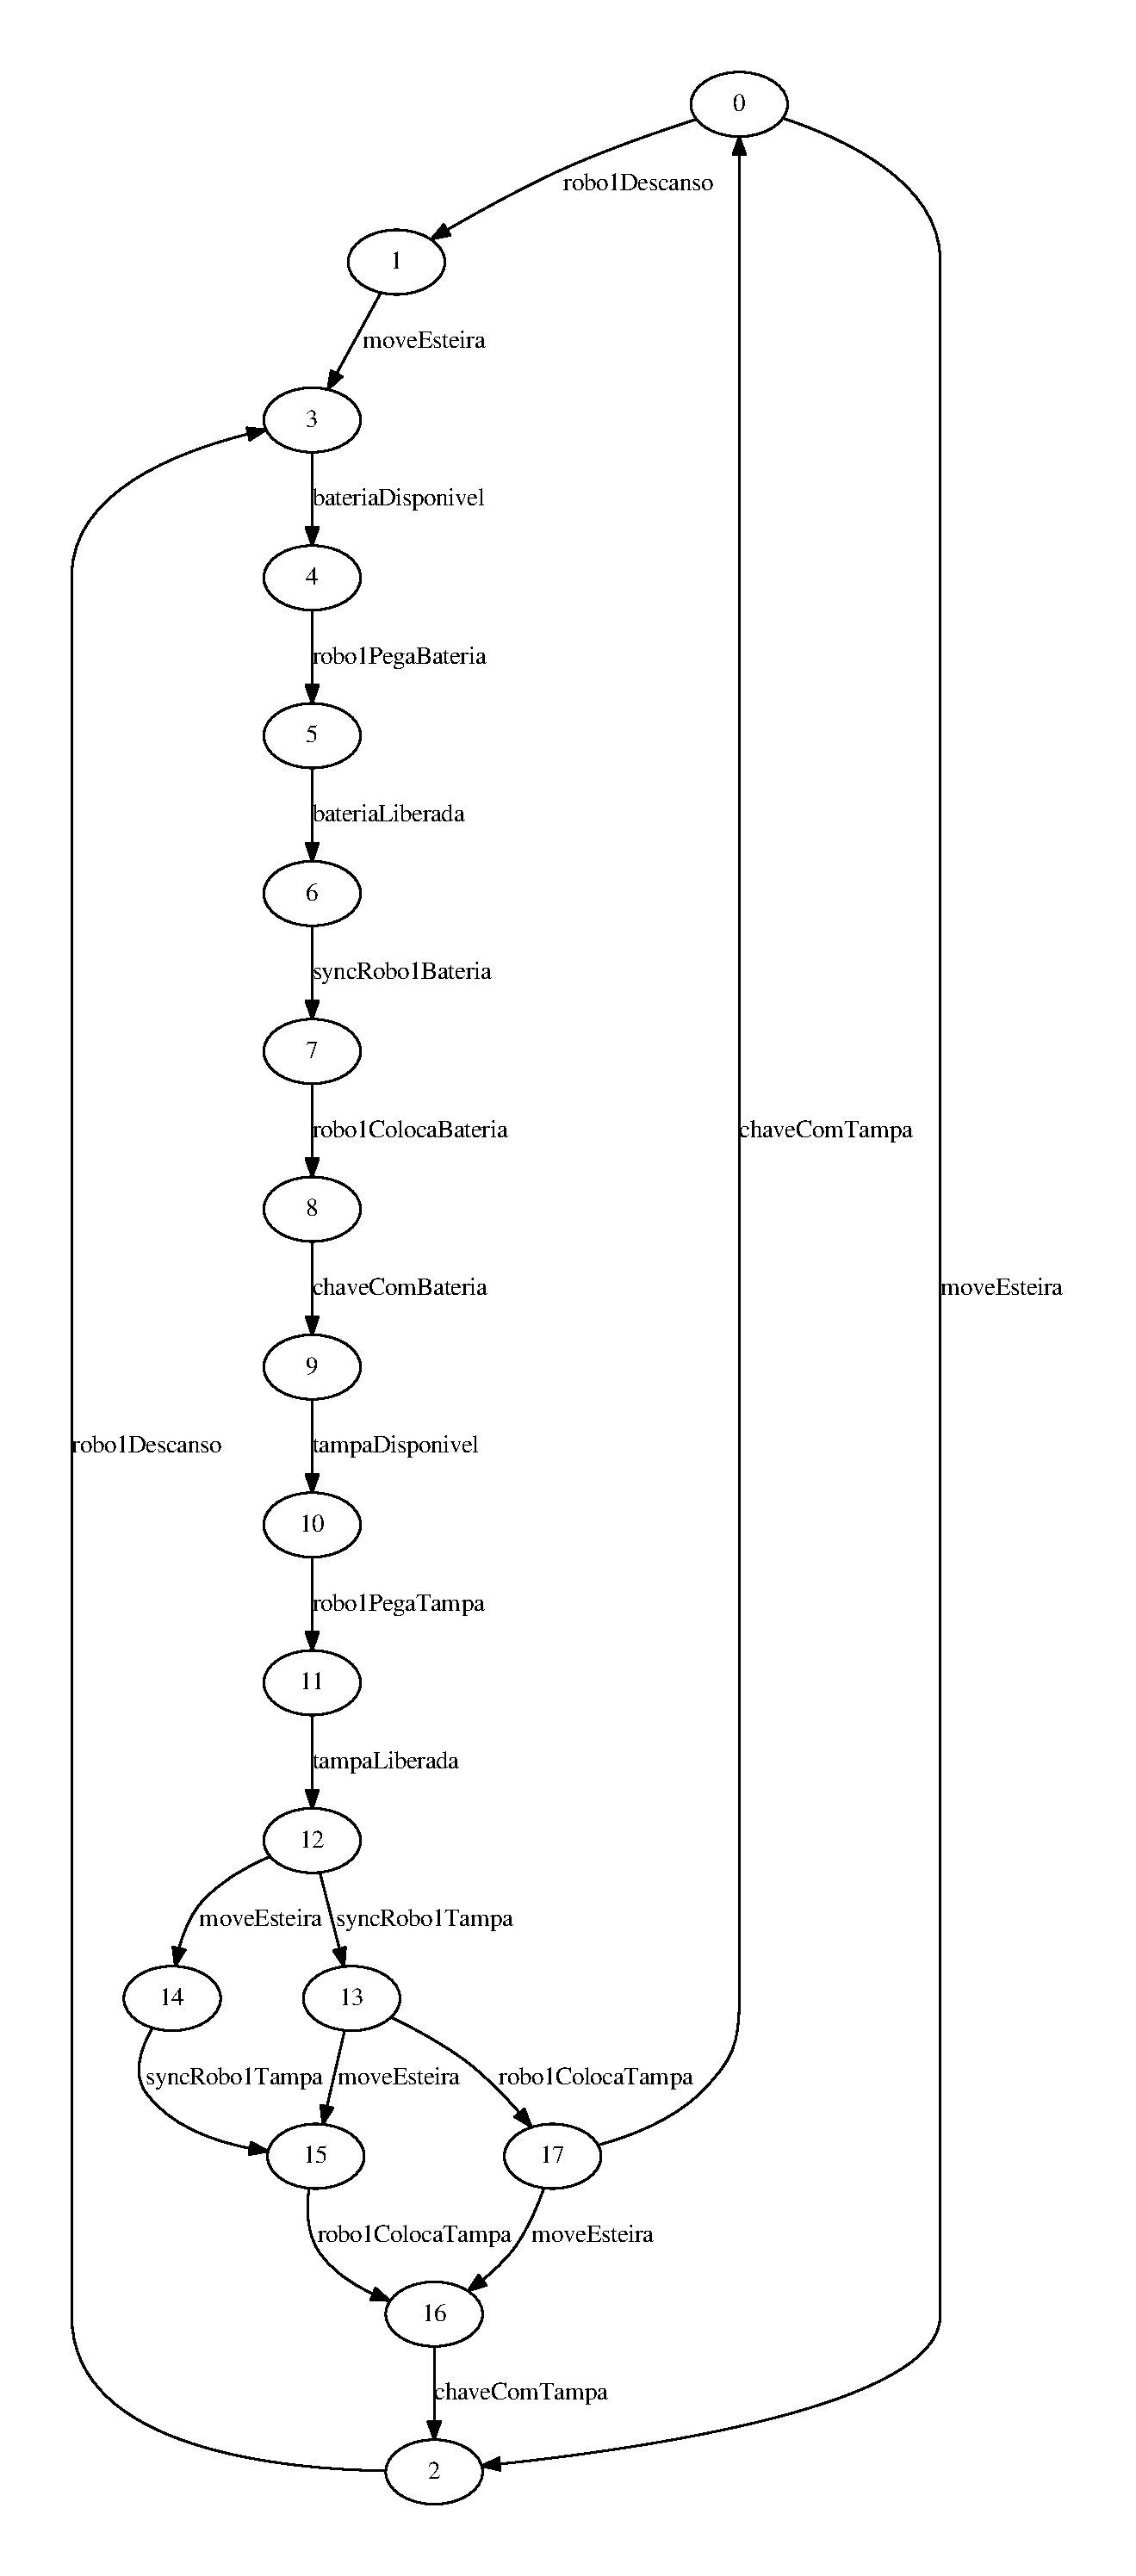
\includegraphics[height = 0.9\textheight]{./img/g_sistema1.pdf}
    \caption{Diagrama subsistema 1 - Robô 1 + Esteira}
    \label{fig:g_subsis1}
\end{figure}

\newpage
\begin{figure}[H]
    \centering
    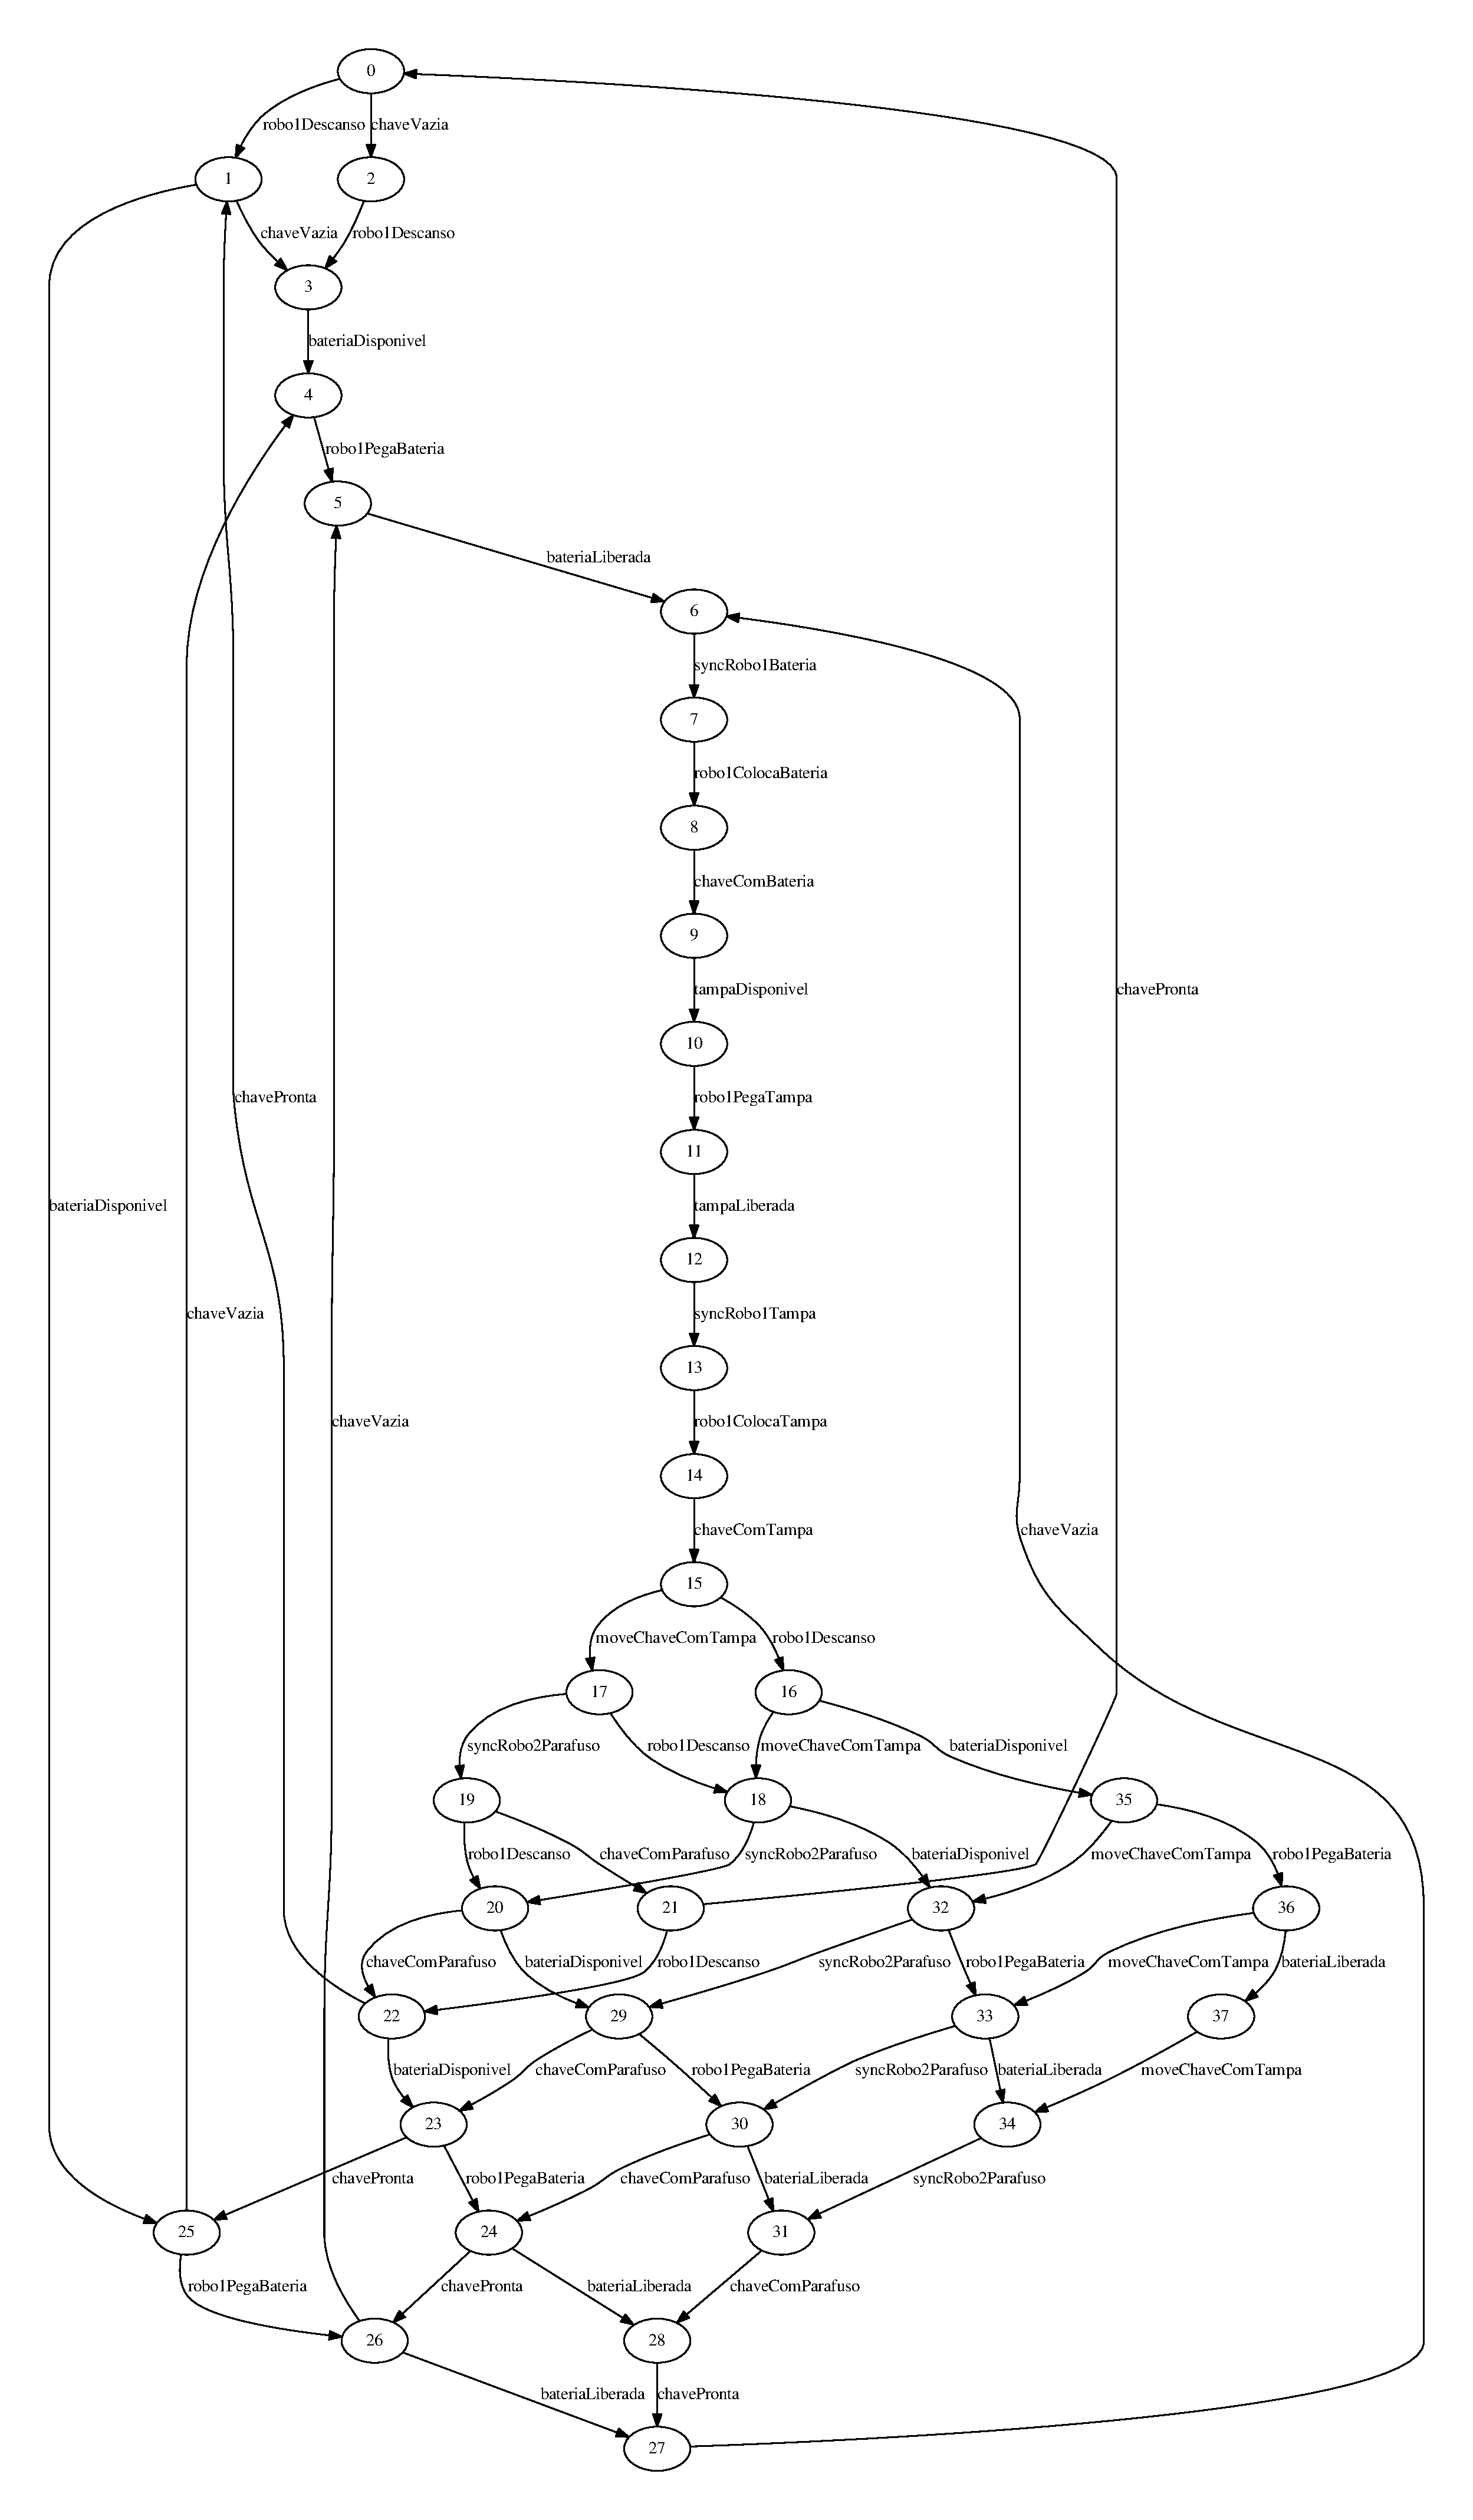
\includegraphics[height = 0.95\textheight]{./img/g_sistema2.pdf}
    \caption{Diagrama subsistema 2 - Robô 1 + Disco}
    \label{fig:g_subsis2}
\end{figure}

\newpage
\begin{figure}[H]
    \centering
    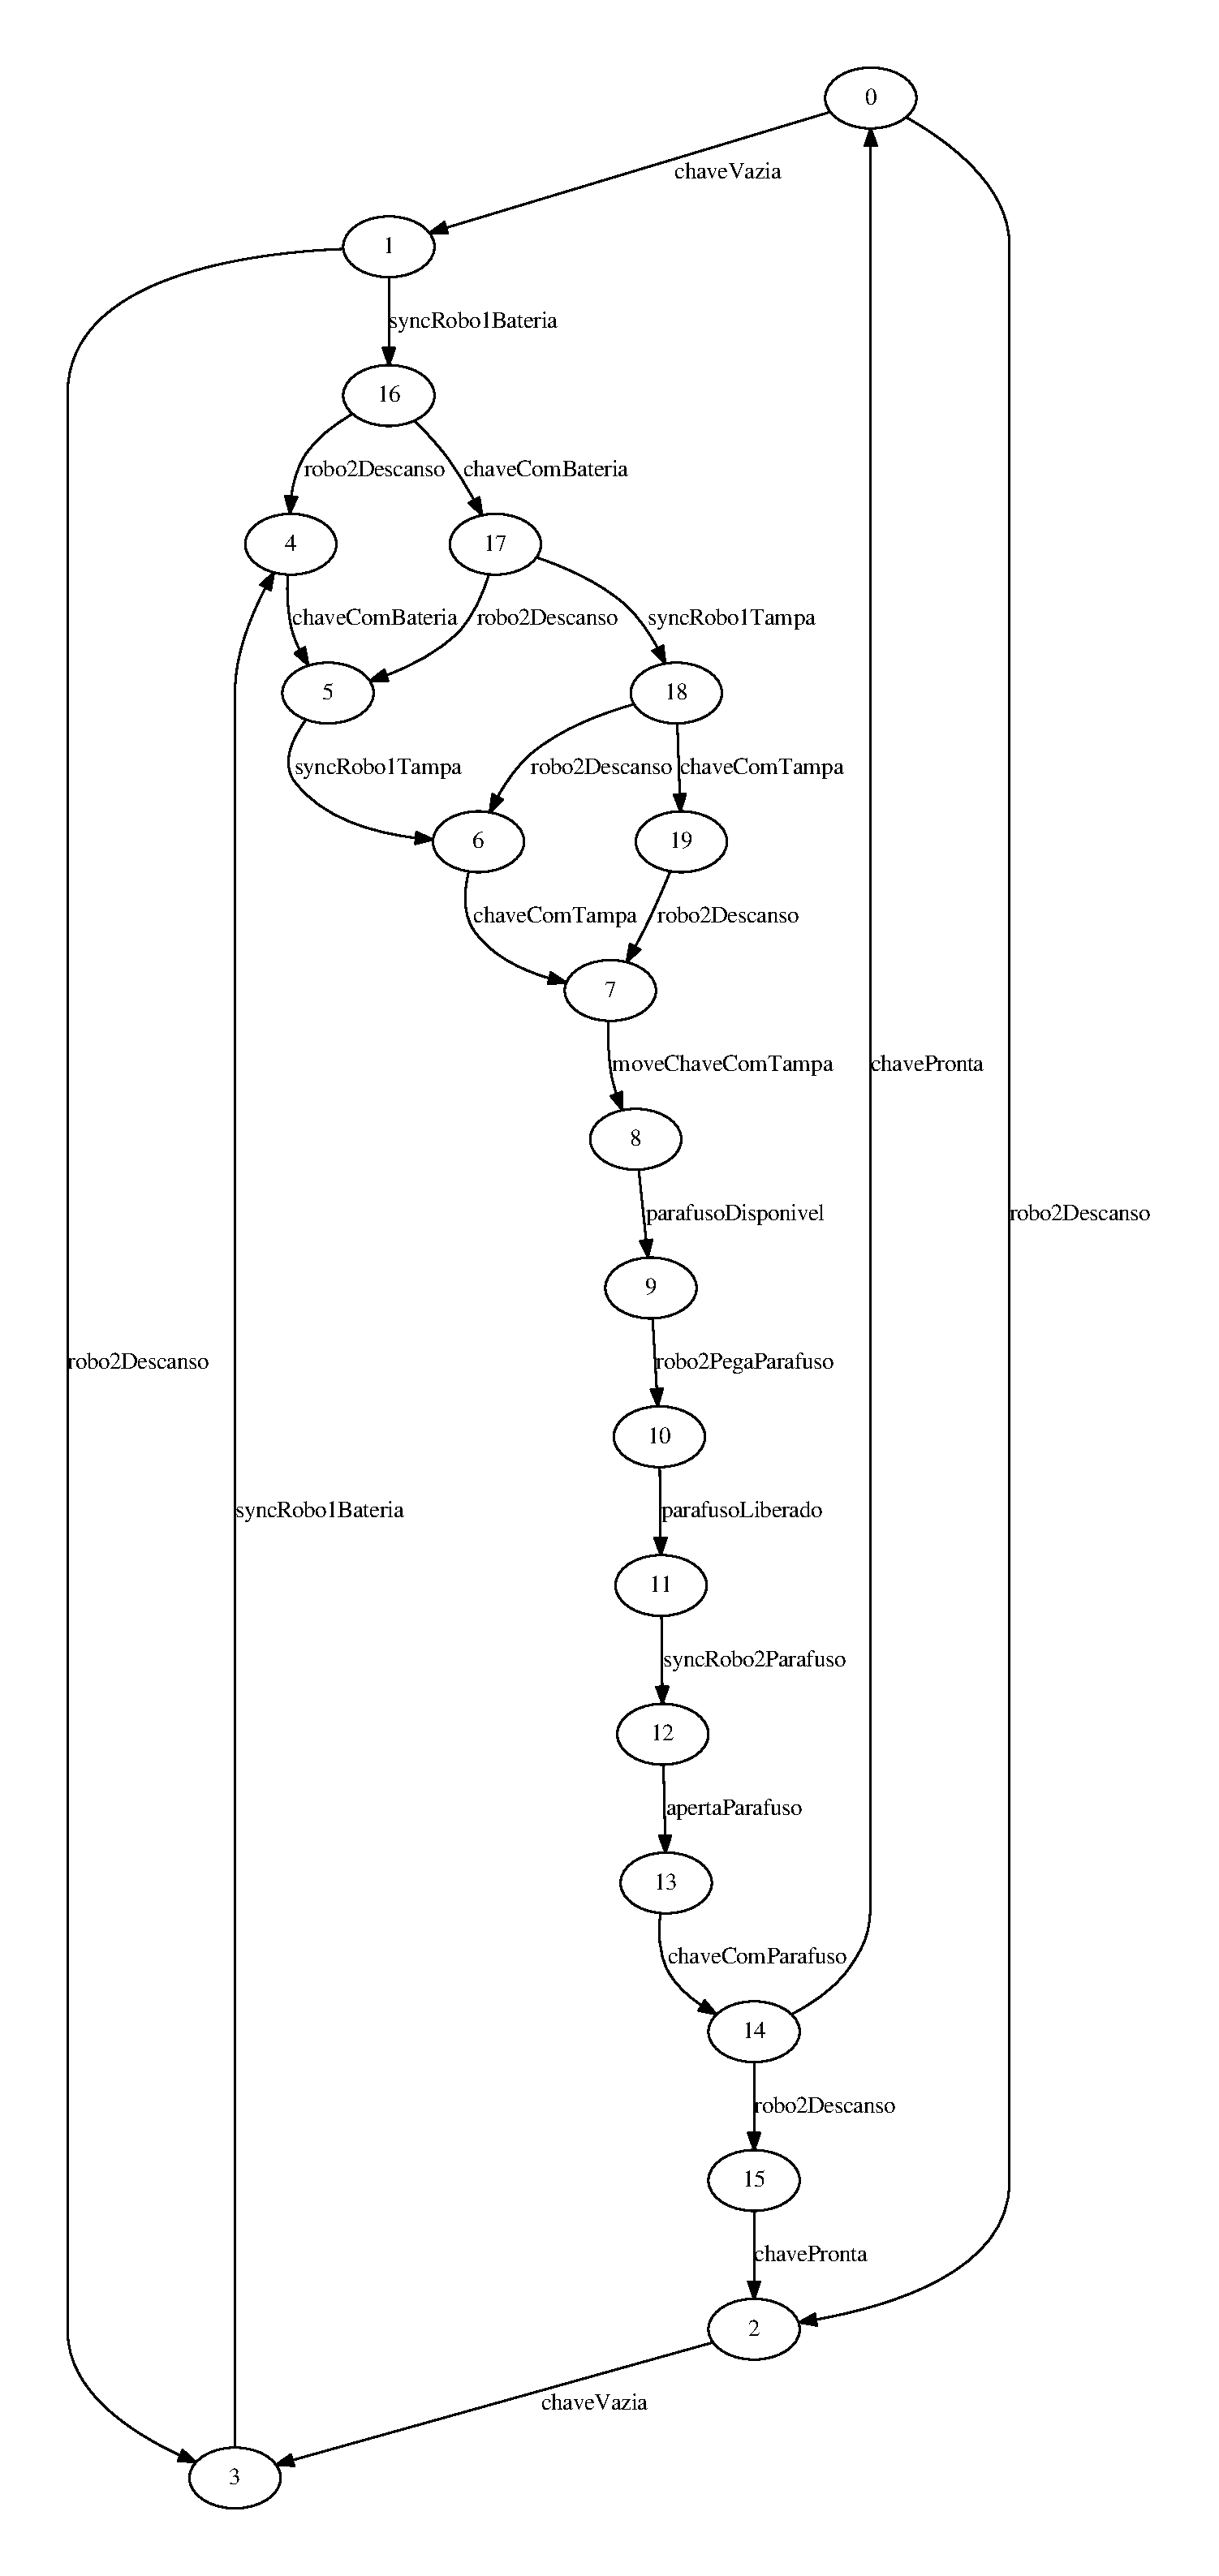
\includegraphics[height = 0.95\textheight]{./img/g_sistema3.pdf}
    \caption{Diagrama subsistema 1 - Robô 2 + Disco}
    \label{fig:g_subsis3}
\end{figure}

\newpage
\begin{figure}[H]
    \centering
    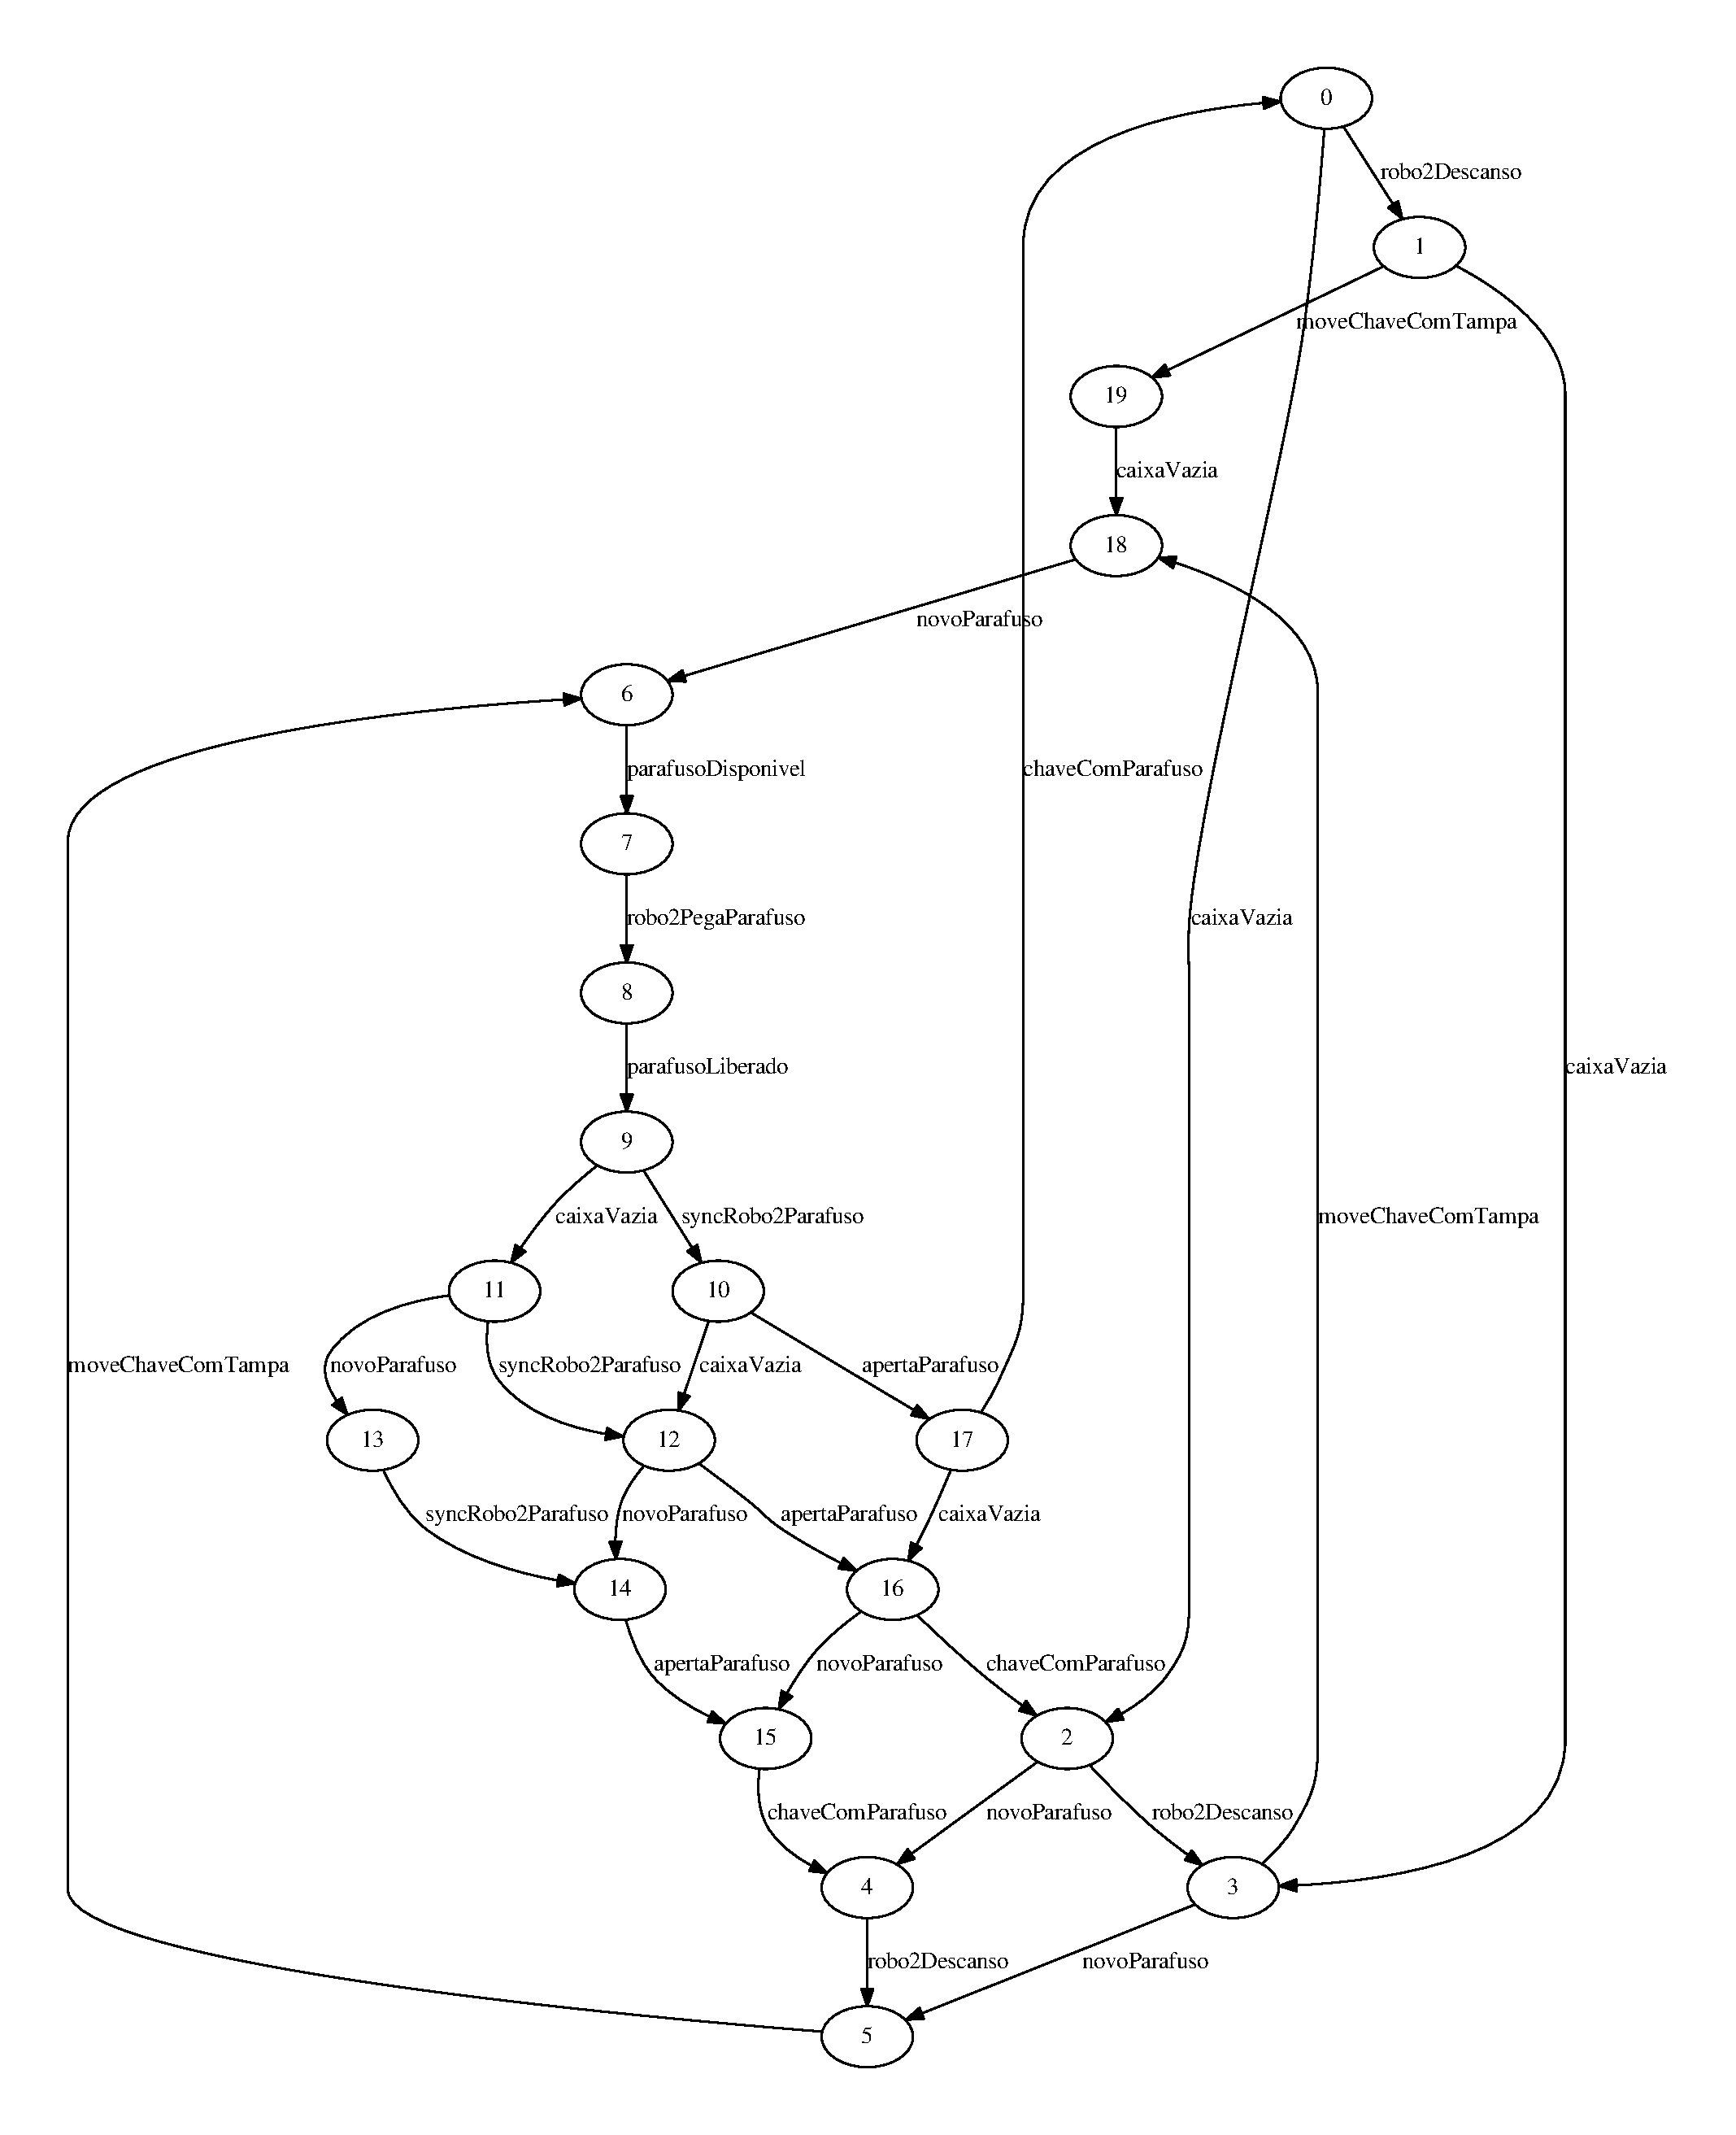
\includegraphics[width = 0.9\linewidth]{./img/g_sistema4.pdf}
    \caption{Diagrama subsistema 1 - Robô 2 + Caixa de Parafusos}
    \label{fig:g_subsis4}
\end{figure}

%%%%%

\newpage
\begin{figure}[H]
    \centering
    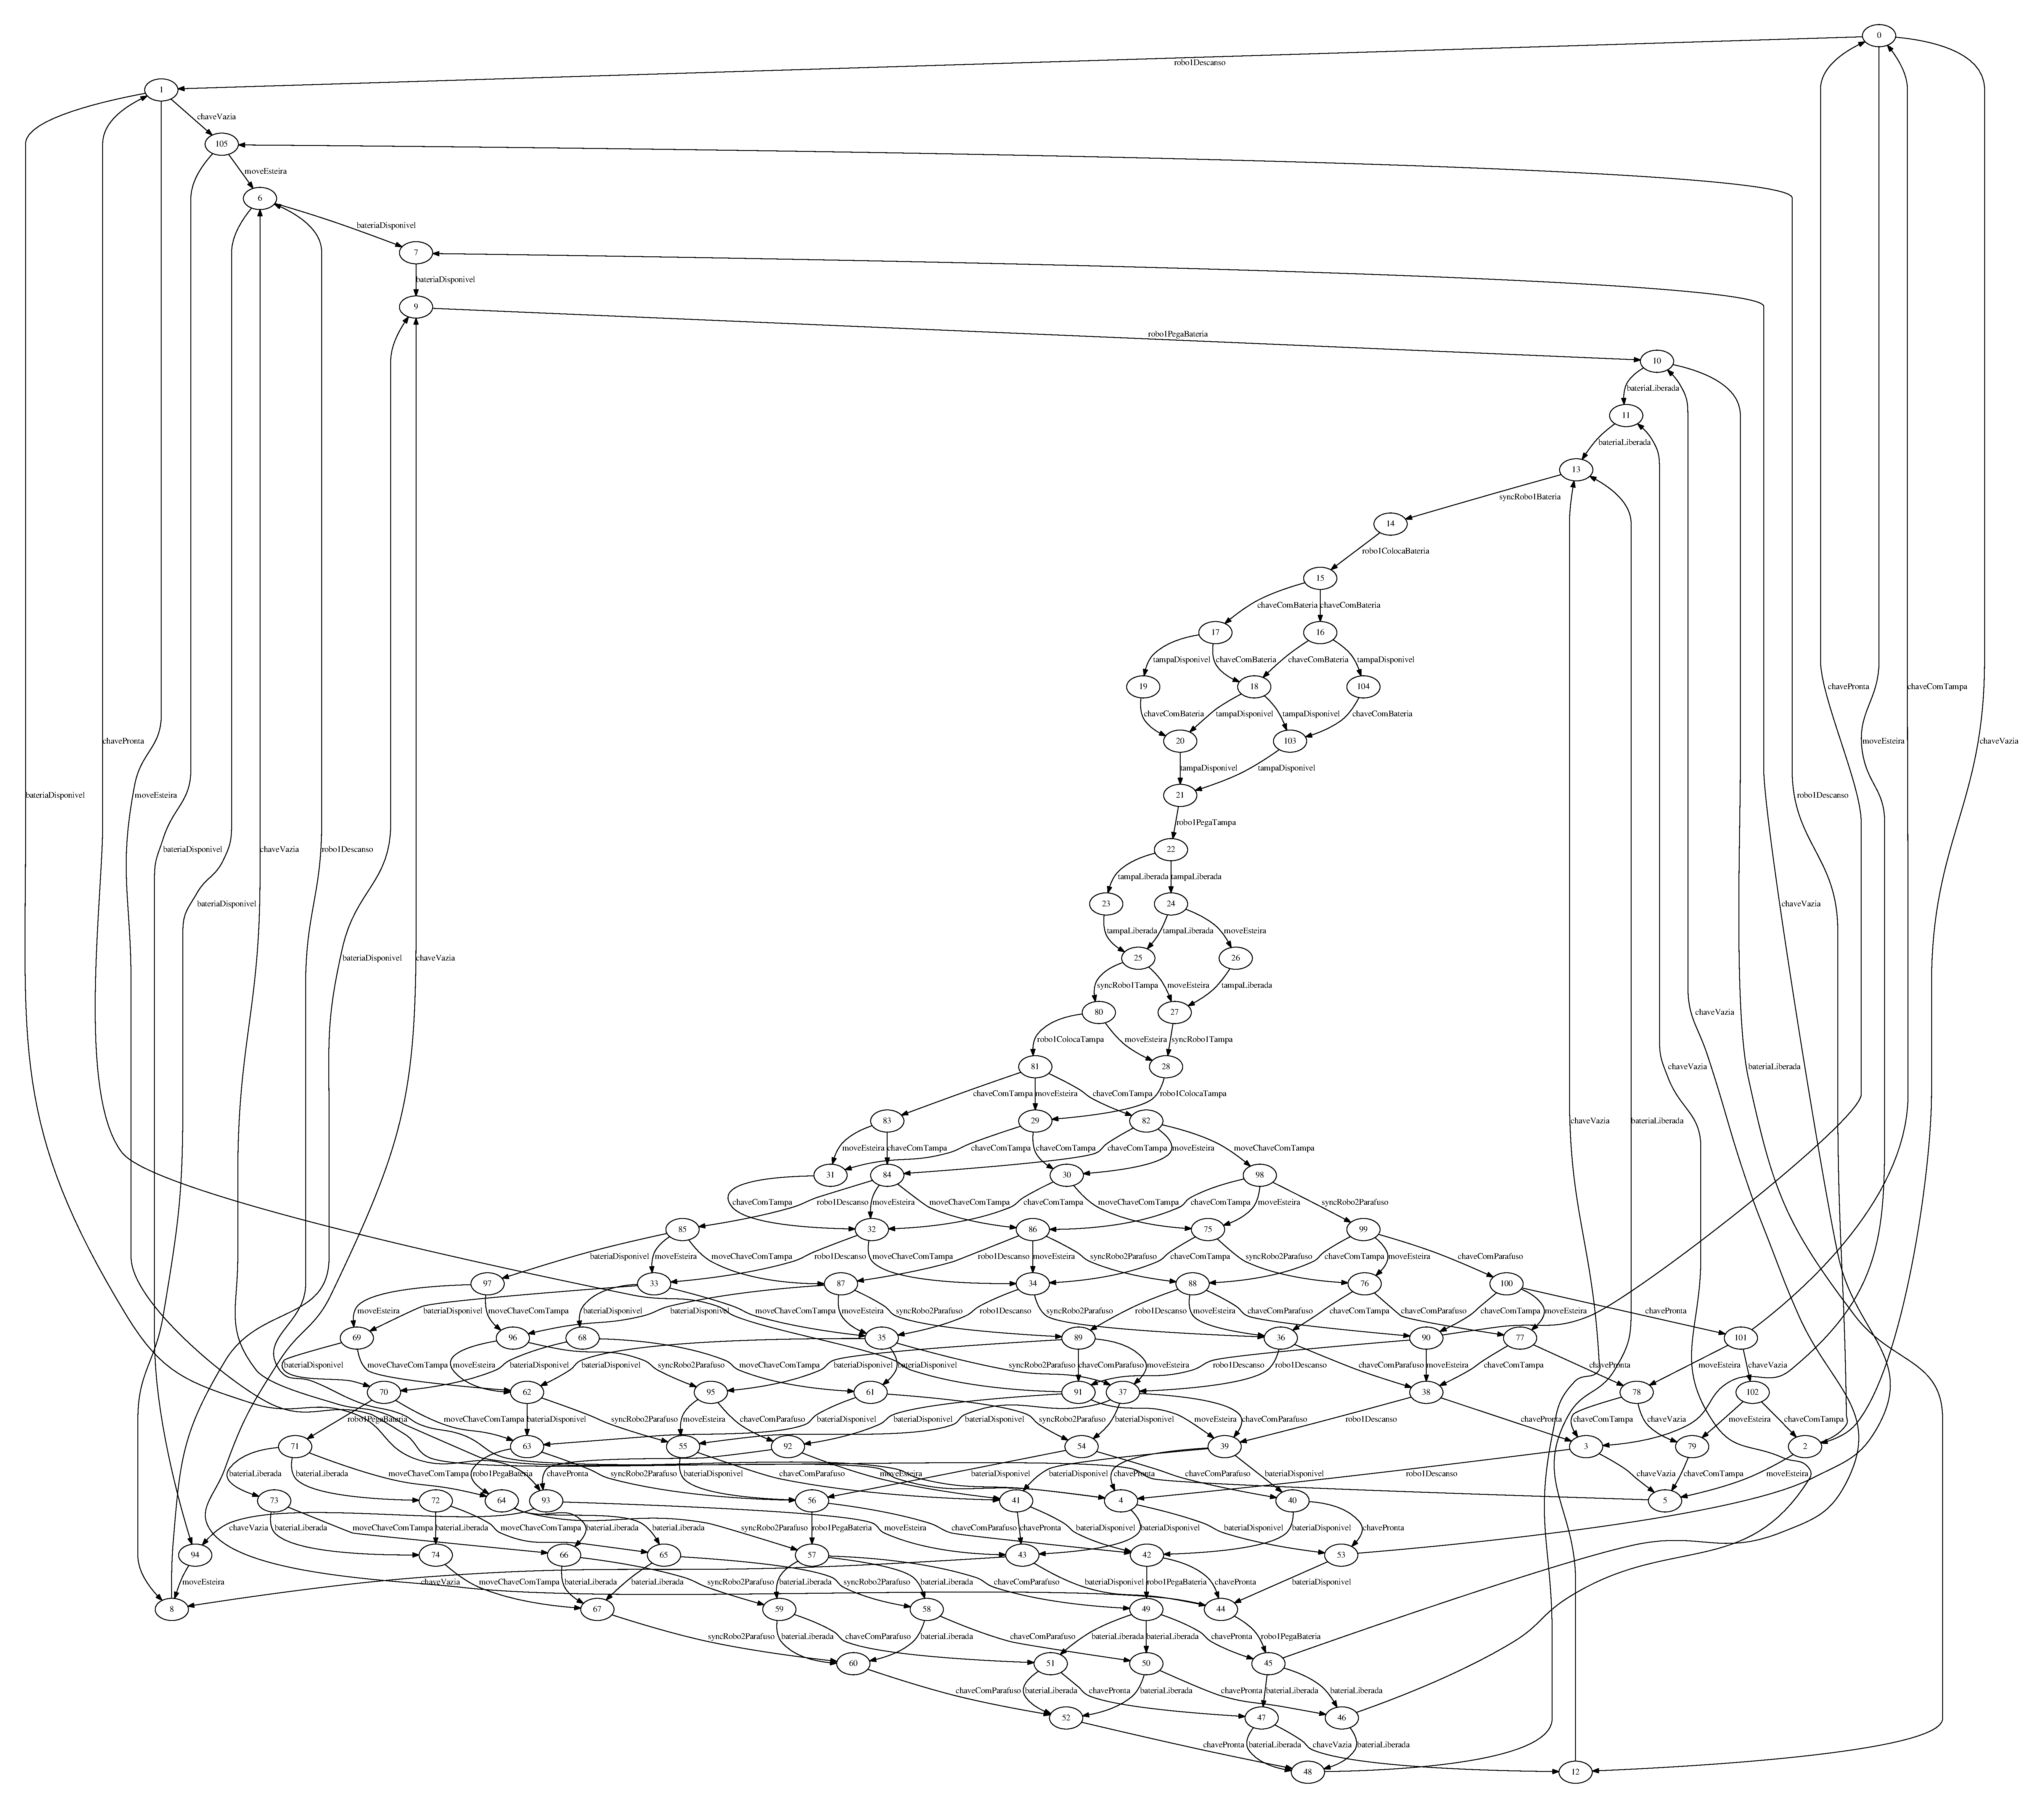
\includegraphics[width = \linewidth]{./img/g_sistema12.pdf}
    \caption{Diagrama subsistema 1 + subsistema 2}
    \label{fig:g_subsis12}
\end{figure}

\newpage
\begin{figure}[H]
    \centering
    \includegraphics[height = 0.95\textheight]{./img/g_sistema23.pdf}
    \caption{Diagrama subsistema 2 + subsistema 3}
    \label{fig:g_subsis23}
\end{figure}

\newpage
\begin{figure}[H]
    \centering
    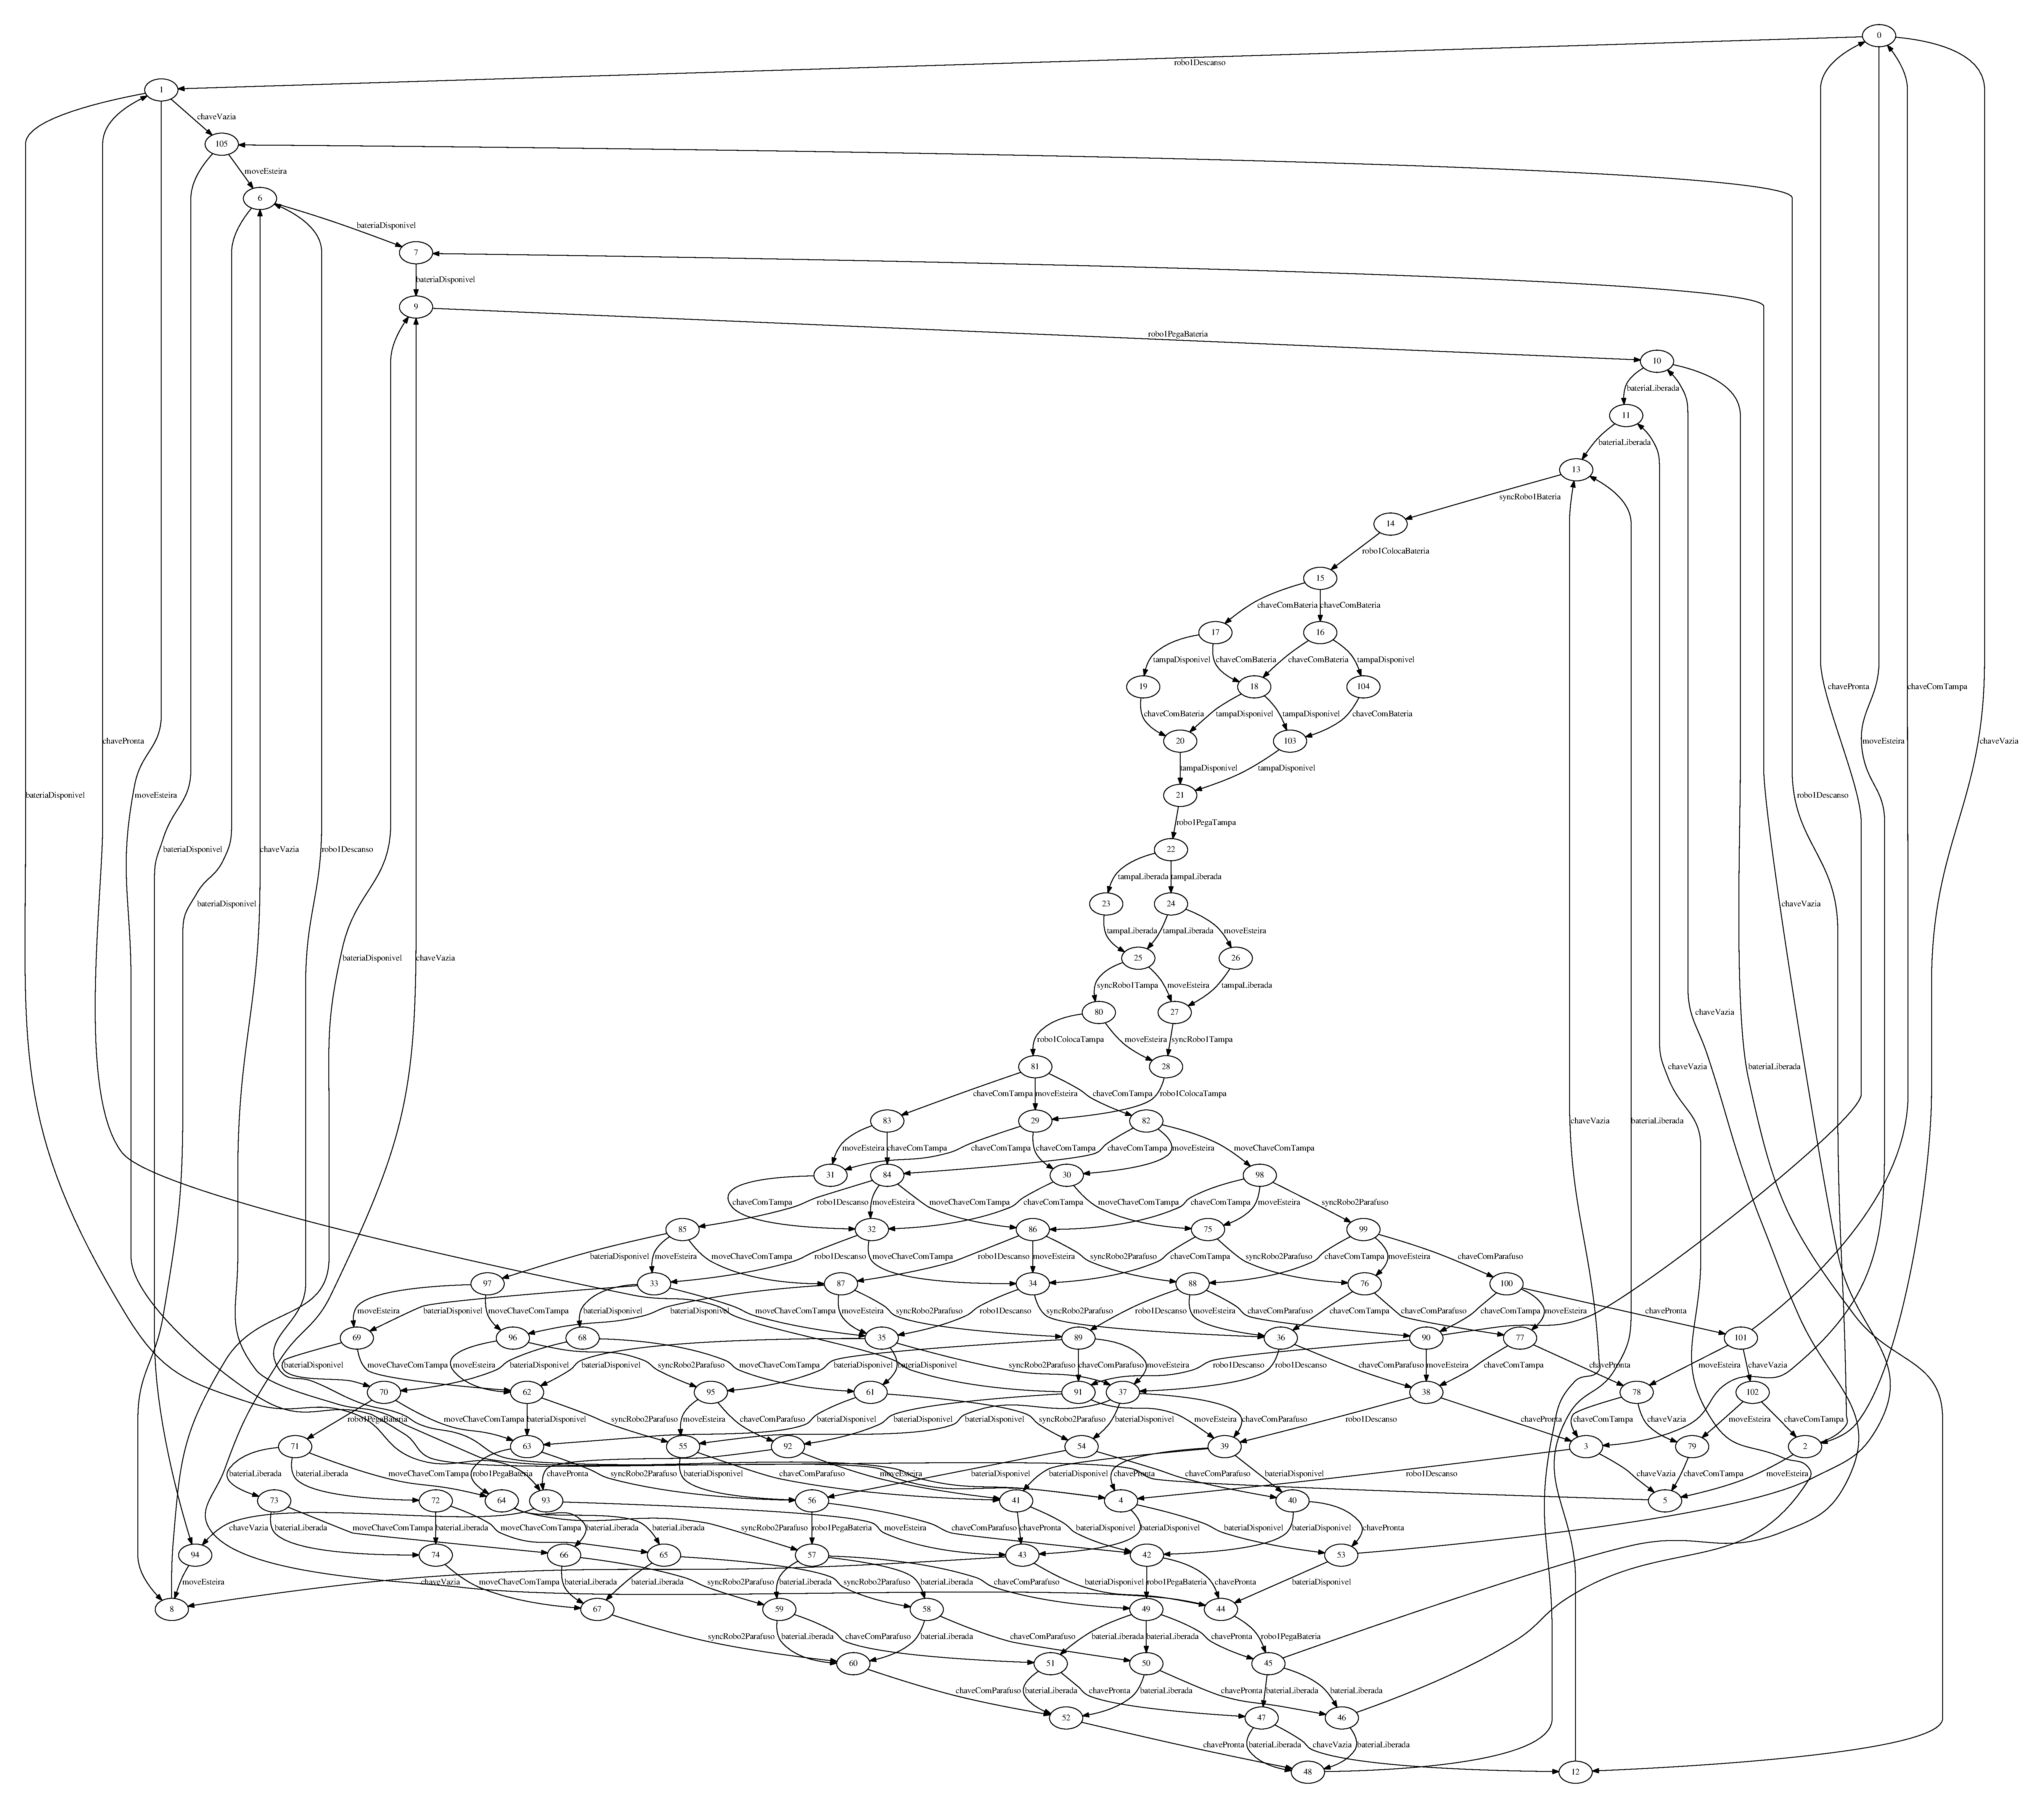
\includegraphics[width = \linewidth]{./img/g_sistema12.pdf}
    \caption{Diagrama subsistema 3 + subsistema 4}
    \label{fig:g_subsis34}
\end{figure}

%%%%%

\newpage
\begin{landscape}
\begin{figure}[H]
    \centering
    \includegraphics[width = \linewidth]{./img/g_sistema.pdf}
    \caption{Diagrama Sistema Completo}
    \label{fig:g_sistema}
\end{figure}
\end{landscape}

\subsection{Verificação de Deadlock}
Uma das grandes facilidades introduzidas pela modelagem em CSP é a possibilidade permitir analises independente da implementação\cite{car.hoare}. No FDR4 esta analises são feitas a partir do comando assert, permitindo testes unitários para caso avaliado. A existência de deadlock para cada subsistema e ao fim para o sistema global, foi verificada a partir dos seguintes comandos:

\begin{minted}[breaklines,frame=single]{lua}
assert SUBSISTEMA1:[deadlock free]
assert SUBSISTEMA2:[deadlock free]
assert SUBSISTEMA3:[deadlock free]
assert SUBSISTEMA4:[deadlock free]
assert SUBSISTEMA12:[deadlock free]
assert SUBSISTEMA23:[deadlock free]
assert SUBSISTEMA34:[deadlock free]
assert SISTEMA:[deadlock free]
\end{minted}

\subsection{Verificando LiveLock}
De maneira similar, a existência de livelock para cada subsistema e ao fim para o sistema global, foi verificada a partir dos seguintes comandos:

\begin{minted}[breaklines,frame=single]{lua}
assert SUBSISTEMA1 :[divergence free]
assert SUBSISTEMA2:[divergence free]
assert SUBSISTEMA3:[divergence free]
assert SUBSISTEMA4:[divergence free]
assert SUBSISTEMA12:[divergence free]
assert SUBSISTEMA23:[divergence free]
assert SUBSISTEMA34:[divergence free]
assert SISTEMA:[divergence free]
\end{minted}

\subsection{Trace}
Ainda foi possível verificar se uma determinada sequências de evento é possível em nosso modelo e assim conferir sequências que trariam problemas, caso viessem a ocorrer. Como exemplo temos a seguinte ordem para o funcionamento da esteira aonde de chegada é trocada:

\begin{minted}[breaklines,frame=single]{lua}
-- Trace Esteira
assert ESTEIRA :[has trace [T]]: <moveEsteira, tampaDisponivel, bateriaDisponivel, tampaLiberada, bateriaLiberada, moveEsteira>
\end{minted}

Note que apesar o processo ESTEIRA permite que a tampa seja pega antes da bateria, a ordem é limitada pelo processo ROBO1. Uma versão alternativa poderia incluir também esta limitação dentro do processo ESTEIRA:

\begin{minted}[breaklines,frame=single]{lua}
ESTEIRA_ = moveEsteira -> bateriaDisponivel -> bateriaLiberada -> tampaDisponivel -> tampaLiberada -> ESTEIRA_
\end{minted}

Neste caso a chegada das peças não seria entendida como processo simultâneos, mas dependentes entre si. O sistema só indicaria que existe uma tampa disponível para o robô 1 pegar se ele já estivesse pego a bateria antes. E neste caso a mesma sequência não será permitida para o modelo.

\begin{minted}[breaklines,frame=single]{lua}
-- Trace Esteira
assert ESTEIRA_ :[has trace [F]]: <moveEsteira, tampaDisponivel, bateriaDisponivel, tampaLiberada, bateriaLiberada, moveEsteira>
\end{minted}


\subsection{Verificação Completa}
O resultado de cada verificação pode ser obtido pela interface gráfica do FDR4 ou ainda diretamente pela linha comando no Linux, através do comando:

\begin{minted}[breaklines,frame=single]{shell}
$ refine -q -b process.csp
\end{minted}

As flags $-q$ e $-b$ foram adicionadas para remover logs de processamento durante o processo de verificação. A partir do qual o comando gerou a seguinte saída:

\begin{minted}[breaklines,frame=single]{shell}
Welcome to FDR Version 4.2.0 copyright 2016 Oxford University Innovation Ltd. All Rights Reserved.
License: Academic license for non-commercial use only
SUBSISTEMA1 :[deadlock free]: Passed
SUBSISTEMA2 :[deadlock free]: Passed
SUBSISTEMA3 :[deadlock free]: Passed
SUBSISTEMA4 :[deadlock free]: Passed
SUBSISTEMA12 :[deadlock free]: Passed
SUBSISTEMA23 :[deadlock free]: Passed
SUBSISTEMA34 :[deadlock free]: Passed
SISTEMA :[deadlock free]: Passed
SUBSISTEMA1 :[divergence free]: Passed
SUBSISTEMA2 :[divergence free]: Passed
SUBSISTEMA3 :[divergence free]: Passed
SUBSISTEMA4 :[divergence free]: Passed
SUBSISTEMA12 :[divergence free]: Passed
SUBSISTEMA23 :[divergence free]: Passed
SUBSISTEMA34 :[divergence free]: Passed
SISTEMA :[divergence free]: Passed
ESTEIRA
    :[has trace [T]] <moveEsteira, tampaDisponivel, bateriaDisponivel,
                      tampaLiberada, bateriaLiberada, moveEsteira>: Passed
ESTEIRA_
    :[has trace [F]] <moveEsteira, tampaDisponivel, bateriaDisponivel,
                      tampaLiberada, bateriaLiberada, moveEsteira>: Failed
\end{minted}

O que permite confirmar que para a implementação feita não foram detectados nenhuma ocorrência de Deadlock para nenhuma das combinações permitidas entre os eventos segundo o modelo implementado.

\section{Conclusão}
O estudo do processo descrito em vídeo permitiu emular a situação de um sistema real junto aos problemas referentes. A descrição em CSP permitiu a análise de situações possíveis ao sistema que não expressas intuitivamente em uma rápida observação e por consequente um aprofundamento no entendimento do sistema. Como exemplo temos os casos em que dois eventos ocorrêm de maneira simultânea, onde a ordem de análise de tais eventos pode provocar situações indesejadas.

A modelagem feita tomou como referência a atitude de cada sistema em relação a chave montada, deste modo é permitido que enquanto o robô 2 esteja finalizando a montagem de uma chave outra esteja sendo montada ao mesmo tempo pelo robô 1. Porém não fornece uma garantia forte que para uma dada chave esta sempre começará como "chave vazia" e terminará como "chave montada", já que entre os robôs 1 e robô 2 não é dado nenhuma dependência de eventos entre si.

Sendo esta restrição necessária, tal dependência poderá ser acrescentada ao modelo como um processo de verificação paralelo ou ainda uma restrição no processo do robô 2 ao invés de depender apenas da restrição imposta pelo evento do processo do disco.

Para trabalhos futuros, novas restrições podem ser incorporadas ao modelo, bem como exceções ao caso do surgimento de eventos inesperados e ainda novos testes unitários poderão ser avaliados partindo dos resultados esperados ao sistema real.

% Referências ----------------------------------------------------------------------------------------------------------------------

\bibliographystyle{plain}
\bibliography{reference}

% https://github.com/jnwhiteh/pygments_csp_lexer
% ----------------------------------------------------------------------------------------------------------------------------------
\end{document}
